% Created 2023-06-28 Wed 11:38
\documentclass[9pt, b5paper]{article}
\usepackage{xeCJK}
\usepackage[T1]{fontenc}
\usepackage{bera}
\usepackage[scaled]{beraserif}
\usepackage[scaled]{berasans}
\usepackage[scaled]{beramono}
\usepackage[cache=false]{minted}
\usepackage{xltxtra}
\usepackage{graphicx}
\usepackage{xcolor}
\usepackage{multirow}
\usepackage{multicol}
\usepackage{float}
\usepackage{textcomp}
\usepackage{algorithm}
\usepackage{algorithmic}
\usepackage{latexsym}
\usepackage{natbib}
\usepackage{geometry}
\geometry{left=1.2cm,right=1.2cm,top=1.5cm,bottom=1.2cm}
\usepackage[xetex,colorlinks=true,CJKbookmarks=true,linkcolor=blue,urlcolor=blue,menucolor=blue]{hyperref}
\newminted{common-lisp}{fontsize=\footnotesize} 
\author{deepwaterooo}
\date{\today}
\title{ET 框架学习笔记(四)--框架总结【爱表哥,爱生活!!!活宝妹就是一定要嫁给亲爱的表哥!爱表哥,爱生活!!!】【活宝妹坐等亲爱的表哥,领娶活宝妹回家!爱表哥,爱生活!!!】}
\hypersetup{
  pdfkeywords={},
  pdfsubject={},
  pdfcreator={Emacs 28.2 (Org mode 8.2.7c)}}
\begin{document}

\maketitle
\tableofcontents


\section{C\# 异步基础原理、状态机原理、逻辑整理}
\label{sec-1}
\subsection{ETVoid C\# Net-async|await 编程更底层一点儿的原理}
\label{sec-1-1}
\begin{itemize}
\item 就是不懂底层的原理是什么,方法定义是什么,返回的是什么,在有 await 等关键字的时候,返回的内容等是如何变换的,以及它背后的那个异步状态机,就是想不明白。
\item 现在参考网上的一个例子,记一下异步任务C\# 幕后封装的那些执行步骤什么的,把 async await 之类的关键字,背后的逻辑理解明白。
\item 就是,可能也可以在异步任务的这个模块,添加无数的日志,通过读日志来把这块儿弄明白。下面就截图网上的这个参考例子。
\begin{minted}[fontsize=\scriptsize,linenos=false]{csharp}
[AsyncMethodBuilder(typeof (AsyncETVoidMethodBuilder))]
internal struct ETVoid: ICriticalNotifyCompletion {
    [DebuggerHidden]
    public void Coroutine() { }
    [DebuggerHidden]
    public bool IsCompleted => true;
    [DebuggerHidden]
    public void OnCompleted(Action continuation) { }
    [DebuggerHidden]
    public void UnsafeOnCompleted(Action continuation) { }
}
\end{minted}
\item 上面是找了一个最短小的类ETVoid, 网上例子自己构建一个类,这个类麻雀虽小五脏俱全的 \textbf{几个【缺一不可】的方法} (所以知道ETTask|ETVoid 自定义封装,这几个方法也是一定不能少的,只是多了Coroutine() 方法不知道是怎么回事儿?)如上如下:
\end{itemize}

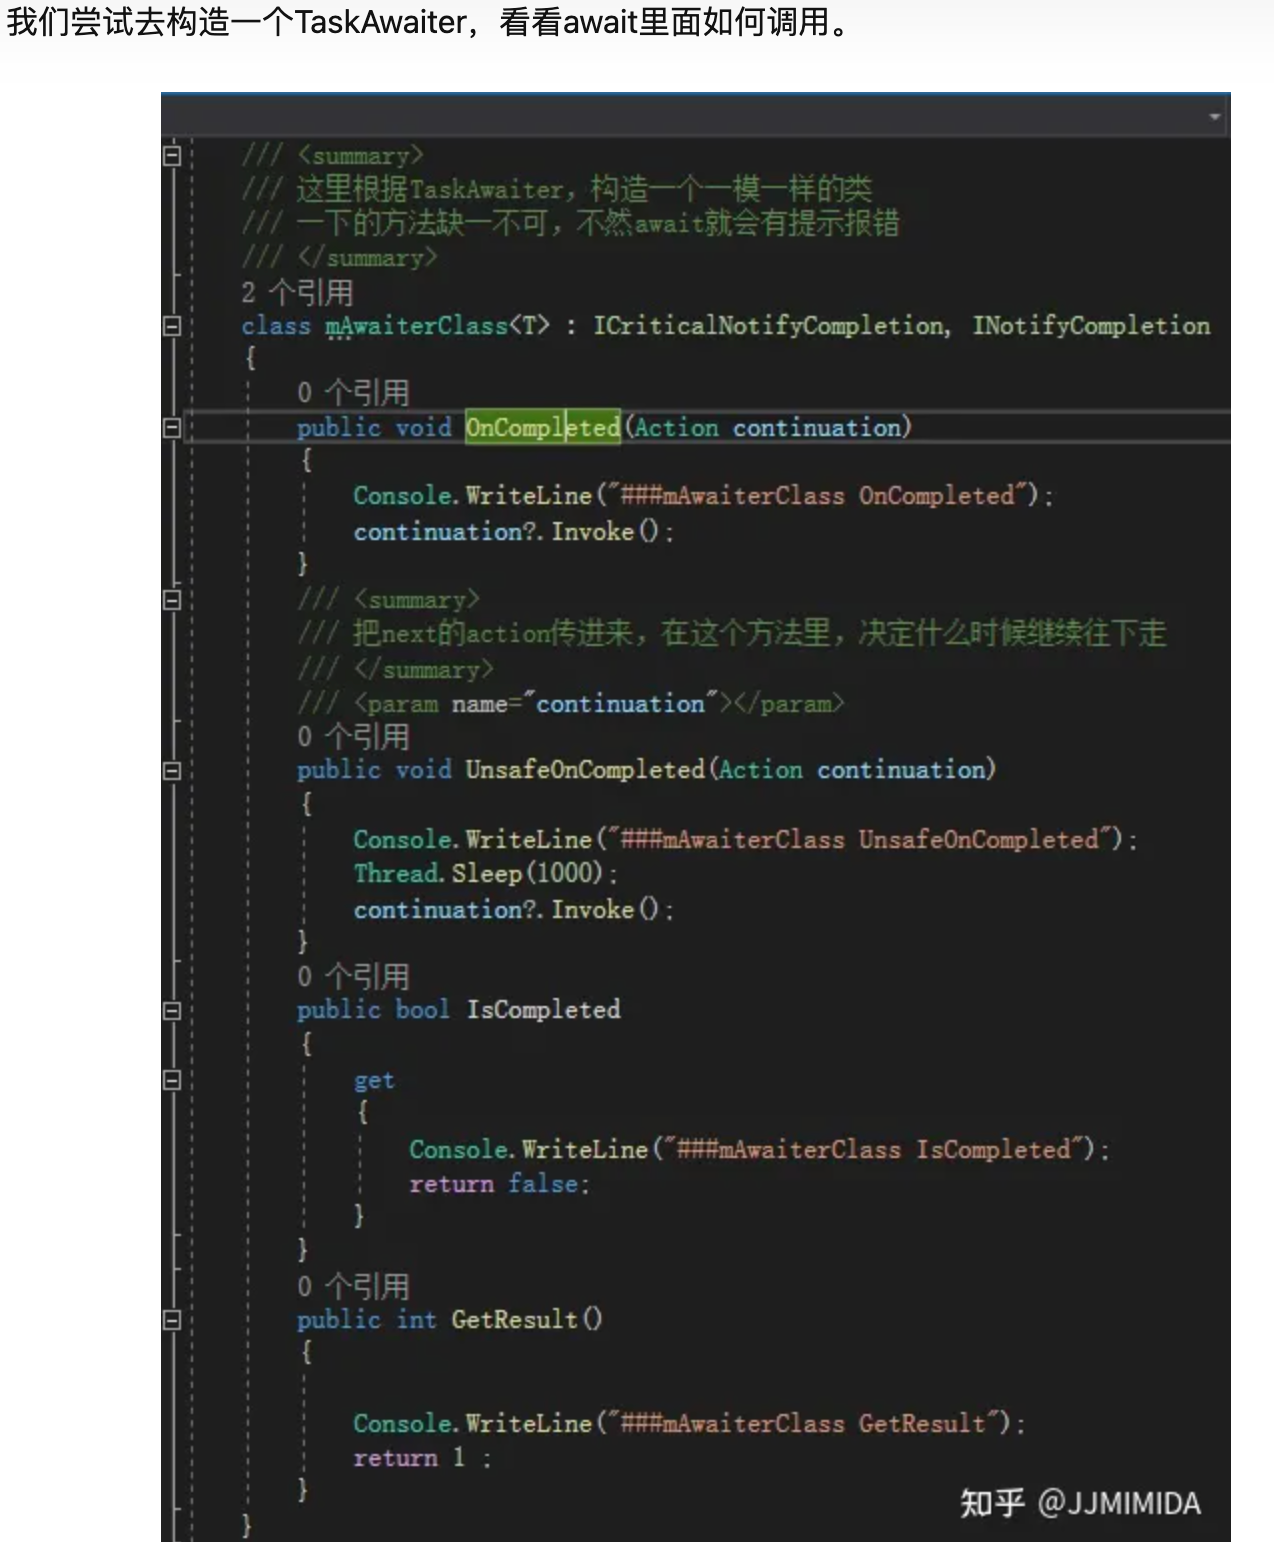
\includegraphics[width=.9\linewidth]{./pic/et3_20230609_105627.png}
\begin{itemize}
\item 它的测试用例是这么写的:注意它传入的参数类型是 int. 后面的编译码里,和它的讲解里会用到提到。
\end{itemize}

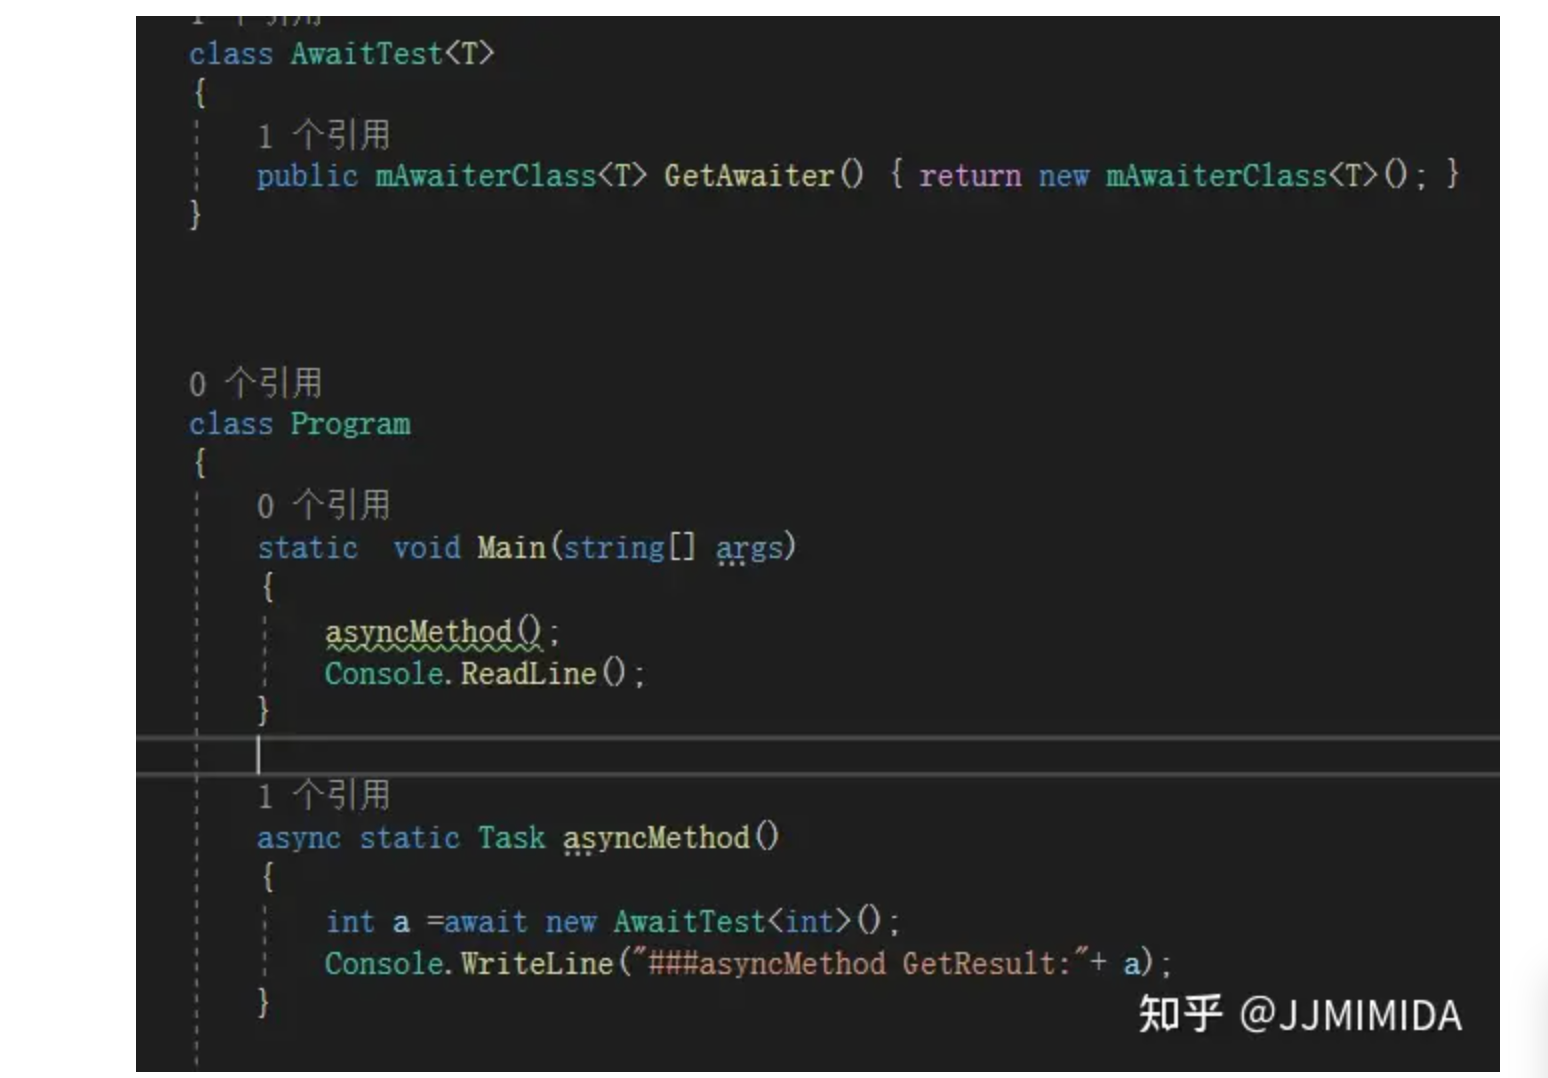
\includegraphics[width=.9\linewidth]{./pic/et3_20230609_105927.png}
\begin{itemize}
\item 看它编译出来的码(那堆编译出来的状态机的码),就是看不懂
\end{itemize}

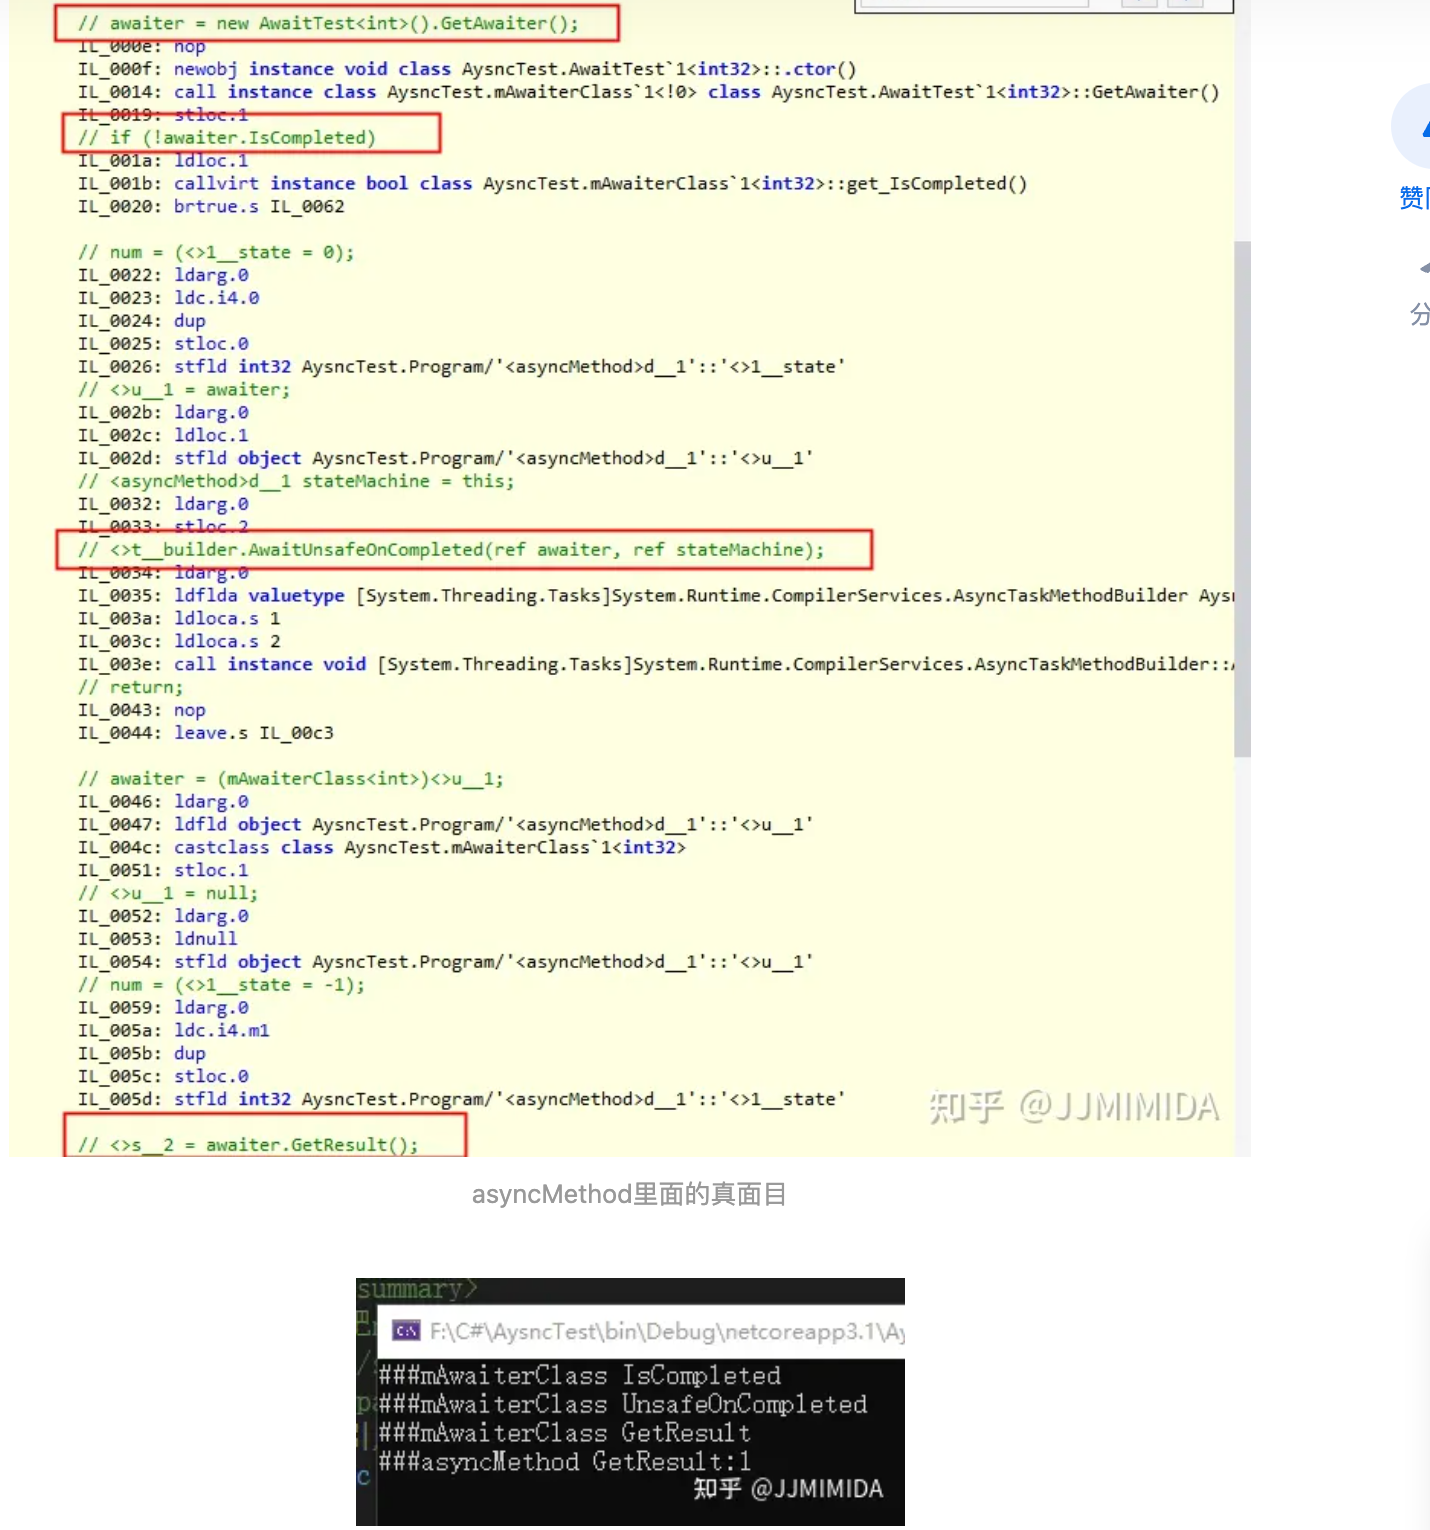
\includegraphics[width=.9\linewidth]{./pic/et3_20230609_112727.png}
\begin{itemize}
\item 结果分析: \textbf{【异步方法状态机,背后的执行顺序与逻辑:】}
\begin{itemize}
\item 先检查IsCompleted标志位,如果已经完成,则调用GetResult作为await的返回值返回。
\item 如果未完成,经过AsyncTaskMethodBuilder的AwaitUnsafeOnCompleted方法之后,最后进入UnsafeOnCompleted(nextAction),并且把完成后的下一步回调传进来。
\item 当我们获得nextAction之后,说明该调用由我们自己来控制,这里我在等待1s之后,执行nextAction(),下一步GetResult返回。
\end{itemize}
\item \textbf{【Async 关键字方法的编译原理:】}
\end{itemize}

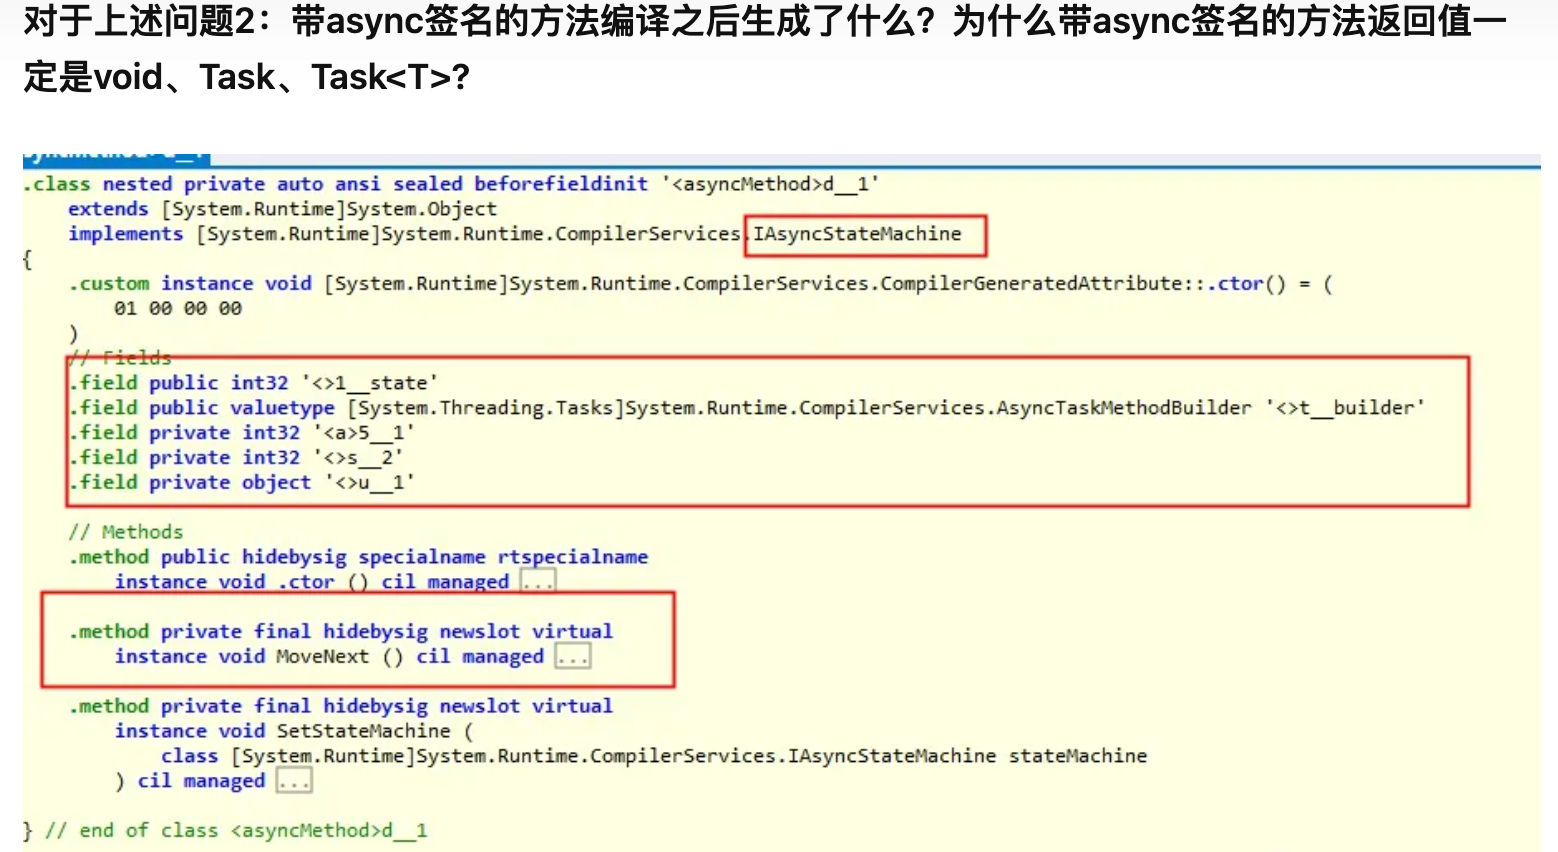
\includegraphics[width=.9\linewidth]{./pic/et3_20230609_110634.png}
\begin{itemize}
\item 这个 async 关键字所标记的异步方法,主要两个点儿: 
\begin{itemize}
\item 编译器,把这个异步方法,编译成了一个类 class <asyncMethod>d\_\_1;
\item 这个类 class, 它实现了 IAsyncStateMachine 接口,( \textbf{实现了这个接口,返回的是什么类型呢?} 这个要想明白?)
\item 这个类 class, 的内部,有几个成员变量 .field-sss.
\item 这个类 class, 的内部,有个特别重要的状态机执行函数 MoveNext() 来指挥指导,异步函数内不同节点如 await 节点等的执行逻辑。 \textbf{【这个类 class, 它实现了 IAsyncStateMachine 接口】}, 前面有列出 IAsyncStateMachine 接口定义的两个方法,所以实现实体类里也会有SetStateMachine() 方法的实现。
\item 上面的逻辑,其实是就是扫描异步方法内,不同的 await 调用,每到一个这个关键字申明的异步调用,就是切换一个状态(背后有可能是线程的切换, 不一定每个分支都用不同的线程,但线程的切换可能是,必要的时候需要切换的?)分段执行。
\end{itemize}
\item 网络上的分析者还给出了下机的截图:不是狠懂,这个截图是什么意思?因为不懂,要把编译码的方法名带上,方便以后再读和理解。
\end{itemize}

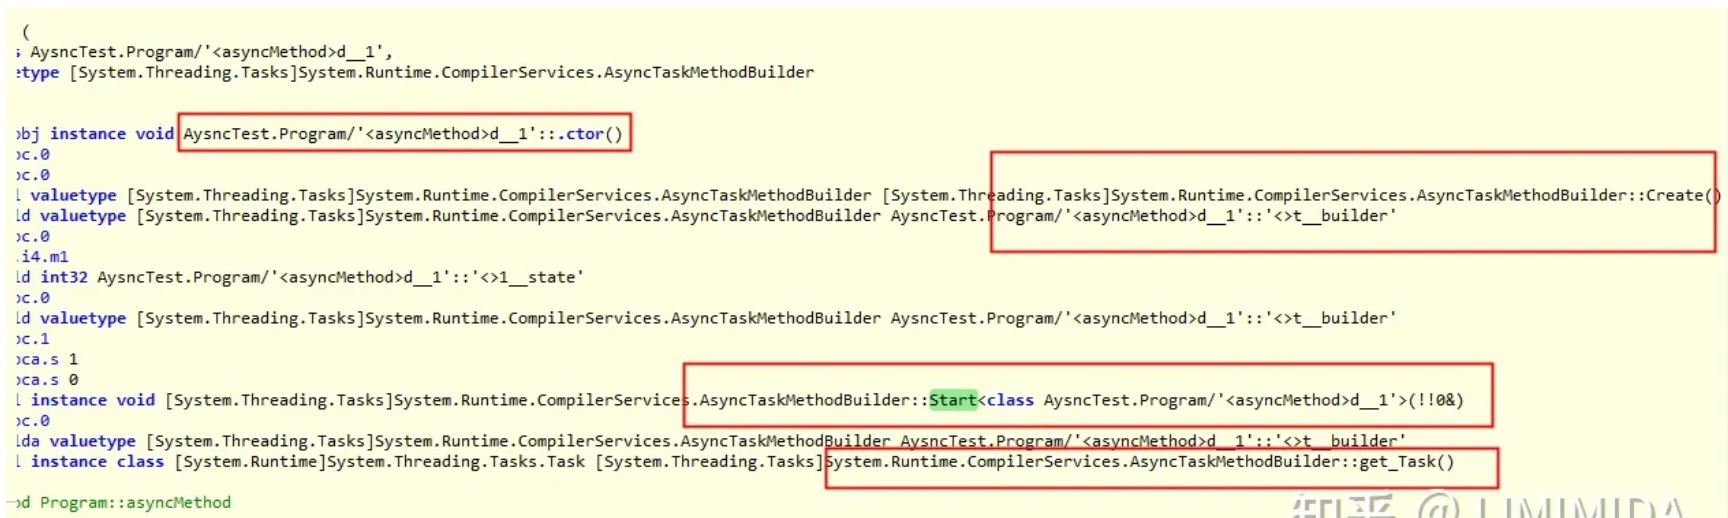
\includegraphics[width=.9\linewidth]{./pic/et3_20230609_112757.png}
\begin{itemize}
\item 上面的异步方法,所生成的异步状态机类 class 里,有几个主要的方法:
\begin{itemize}
\item 构造器方法 ctor():
\item Create() 方法:
\item Start() 方法:
\item get\_Task() 方法:
\end{itemize}
\item 可是上面的几个方法是谁,哪个接口定义的呢?
\item 网络上的分析者,对上面两个截图的分析如下: \textbf{【它讲解的这部分,我可能还是得自己编译一下,去具体看一下。】因为它的截图不完整,看不懂} 下面还有个别人总结的状态机套路,感觉说得更彻底透彻。
\begin{itemize}
\item 签名为async Task asyncMethod()的方法里,先创建一个继承自IAsyncStateMachine的asyncMethod类
\item 创建一个AsyncTaskMethodBuilder,然后赋值给Machine. (不知道,它这句,说的是哪里?第一个图的最后 SetStateMachine()?)
\item 初始化Machine的state = -1. (两个截图里看不见,找不到)
\item 调用AsyncTaskMethodBuilder.Start方法,start里面会进入Machine的moveNext()方法,详见问题1。
\item AsyncTaskMethodBuilder.get\_Task() 作为该方法的返回值返回。
\end{itemize}
\item 多线程问题: Task一定是多线程吗?
\begin{itemize}
\item 不一定,在上述例子中,我们定义的 async static Task<int> aa(),里面就是在同一个线程执行的。只有调用Task.Start 或者Task.Run 里面自动启用多线程的时候,才是多线程。
\end{itemize}
\item 看得另一个网页中的说法,因为感觉它也没有实现个什么公共定义约束的接口,理解得不够透彻。看下下面的:
\item await 必须配合 Task/ValueTask 才能用吗?当然不是。
\begin{itemize}
\item 在 C\# 中 \textbf{只要你的类中包含 GetAwaiter() 方法和 bool IsCompleted 属性,并且 GetAwaiter() 返回的东西包含一个 GetResult() 方法、一个 bool IsCompleted 属性和实现了 INotifyCompletion,那么这个类的对象就是可以 await 的} 。这里说得还是不清楚,不透彻,换一个表达得更清晰的说法如下:
\end{itemize}
\item 可以使用await的方法,返回值必须是 \textbf{awaitable对象} ,自定义awaitable对象比较麻烦,一个对象必须满足下列条件才行:
\begin{itemize}
\item 必须有一个 \textbf{GetAwaiter()} 方法,扩展方法或者实例方法都可以
\item GetAwaiter() 方法返回值必须是 \textbf{awaiter对象} 。一个对象要成为awaiter对象必须满足下列条件:
\begin{itemize}
\item 该对象 \textbf{实现接口 INotifyCompletion 或者ICriticalNotifyCompletion}
\item 必须有 \textbf{IsCompleted属性}
\item 必须有 \textbf{GetResult()方法} ,可以返回void或者其他返回值。
\end{itemize}
\end{itemize}
\item 比如下面的自定义类:把几个类的本质理解得再深一点儿了吗?【爱表哥,爱生活!!!任何时候,活宝妹就是一定要嫁给亲爱的表哥!!!】
\end{itemize}
\begin{minted}[fontsize=\scriptsize,linenos=false]{csharp}
public class MyTask<T> {
    public MyAwaiter<T> GetAwaiter() {// 必须提供的方法 
        return new MyAwaiter<T>();
    }
}
// 下面自定义的类 MyAwaiter<T=亲爱的表哥> 就是可以 await 的:
// 【任何时候,活宝妹就是一定要嫁给亲爱的表哥!!!活宝妹还没能嫁给亲爱的表哥,活宝妹就是永远守候在亲爱的表哥的身边!!!爱表哥,爱生活!!!】
public class MyAwaiter<T> : INotifyCompletion {// 必须实现的接口
    public bool IsCompleted { get; private set; }// 属性变量 
    public T GetResult() {// 必须要有的方法 
        throw new NotImplementedException();
    }
    public void OnCompleted(Action continuation) {
        throw new NotImplementedException();
    }
}
public class Program {
    static async Task Main(string[] args) {
        var obj = new MyTask<int>();
        await obj;
    }
}
\end{minted}
\begin{itemize}
\item \textbf{【状态机套路】:}
\item async关键字标记方法是一个异步方法,编译器通过这个标记 \textbf{【async关键字】} 去改造这个方法体为创建状态机的方法。await是关键字,是为了实现状态机中的一个状态, 每当有一个await,就会生成一个对应的状态。状态机就是根据这个状态,去一步步的调用异步委托,然后回调,包括状态机的解析。
\item (1).状态机的默认状态都是-1, 结束状态都是-2.
\item (2).每await一次就会产生一个 TaskAwaiter awaiter; 改变状态机的状态, 当有多个await的时候,每个await都会改变状态机的状态,比如 改为 0,1,2,3,4 等等, 分别表示代码中await xxx 这句话执行完成。
\item (3).状态机的执行套路:
\begin{itemize}
\item A. 首先创建一个 d\_num 的方法(这里说错了,应该是创建了一个类 class), xxx代表方法名,num可能是0,1,2,3等, \textbf{实现IAsyncStateMachine接口。}
\item B. 在MoveNext()方法中, 源代码中每个 await xxxx 都会对应生成是一个 TaskAwaiter awaiter,然后 xxxx.GetAwaiter()
\item C. 判断状态机是否执行完if (!awaiter.IsCompleted),
\begin{itemize}
\item 没有执行完的话走 <>t\_\_builder.AwaitUnsafeOnCompleted(ref awaiter, ref stateMachine); 代表释放当前线程
\item 执行完后走,<>s\_\_1 = awaiter.GetResult(); 拿到返回值,继续走后面的代码。
\end{itemize}
\end{itemize}
\item (此处写的比较抽象,看下面3 结合代码编译再分析)
\item 感觉今天读这个状态机:\url{https://linuxcpp.0voice.com/?id=1380} 终于有点儿开窃了!!【爱表哥,爱生活!!!任何时候,活宝妹就是一定要嫁给亲爱的表哥!!!爱表哥,爱生活!!!】
\end{itemize}
\subsection{如果方法声明为 async,那么可以直接 return 具体的值,不再用创建Task,由编译器创建 Task:}
\label{sec-1-2}
\begin{minted}[fontsize=\scriptsize,linenos=false]{csharp}
// 只要标记了async 就会被编译成状态机
// 如果方法声明为 async,那么可以直接 return 具体的值,不再用创建Task,由编译器创建 Task: 
  public static async Task<int> F2Async() {
      return 2;
  }
\end{minted}
\begin{itemize}
\item F2Async:只加了async,会生成状态机,但由于没有加await所以不会涉及到中间状态的变化,从-1默认状态 变为 结束的-2状态。
\end{itemize}
\begin{itemize}
\item F3Async:既有async也有await (await只有1个),该方法是使用了Task.Run,我们把它归为计算型的异步方法。
\item 亲爱的表哥,活宝妹今天终于把这个看得稍微有点儿懂了,希望能够赶快从这个ETTask 模块 move-forward. 任何时候,活宝妹就是一定要嫁给亲爱的表哥!!!活宝妹还没能嫁给亲爱的表哥,活宝妹就是永远守候在亲爱的表哥的身边!!!爱表哥,爱生活!!!
\end{itemize}


\section{Protobuf 相关,【Protobuf 里进程间传递的游戏数据相关信息:两个思路】}
\label{sec-2}
\begin{itemize}
\item 【一、】查找 enum 可能可以用系统平台下的 protoc 来代为生成,效果差不多。只起现 Proto2CS.cs 编译的补充作用。
\item 【二、】Card 类下的两个 enum 变量,在ILRuntime 热更新库下,还是需要帮它连一下的。用的是 HybridCLR
\item 【三、】查找 protoc 命令下,如何C\# 索引 Unity 第三方库。
\item 【四、】repeated 逻辑没有处理好
\begin{minted}[fontsize=\scriptsize,linenos=false]{csharp}
message Actor_GamerPlayCard_Req // IActorRequest
{
	int32 RpcId = 90;
	int64 ActorId = 91;
    repeated ET Card Cards = 1;
}
\end{minted}
\item 【Windows 下的 Protobuf 编译环境】:配置好,只是作为与ET 框架的Proto2CS.cs 所指挥的编译结果,作一个对比,两者应该效果是一样的,或是基本一样的,除了自定义里没有处理 enum.
\item Windows 下的命令行,就是用 protoc 来编译,可以参考如下. (这是 .cs 源码下的)
\begin{minted}[fontsize=\scriptsize,linenos=false]{csharp}
CommandRun($"protoc.exe", $"--csharp_out=\"./{outputPath}\" --proto_path=\"{protoPath}\" {protoName}");
\end{minted}
\item 现在的问题是, \textbf{Protobuf消息里面居然是有 unity 第三方库的索引} 。
\item 直接把 enum 生成的那三个 .cs 类分别复制进双端,服务器端与客户端。包括Card 类。那些编译错误会去天边。哈哈哈,除了一个Card 的两个变量之外(CardSuits, CardWeight)。
\item 【热更新库】:现在剩下的问题,就成为,判定是用了哪个热更新的库,ILRuntime, 还是 HybridCLR, 如果帮它连那两个变量。好像接的是 HybridCLR. 这个库是我之前还不曾真正用过的。
\begin{itemize}
\item 相比于ET6,彻底剔除了ILRuntime,使得代码简洁了不少,并且比较稳定
\end{itemize}
\end{itemize}


\section{Unit: 这个模块还不太懂,需要明天上午花时间再看一下}
\label{sec-3}
\begin{itemize}
\item 【Unit】究竟是什么:感觉像是视图里的控件的基本单位?它带位置、旋转信息
\item 有个编译错误说:这个组件不可以同时成分多于一个不同组件组成元件。。。可是框架中使用的地方,明明把它添加进了不同的组件。去弄明白框架里,如何控件一个组件只能成为一个【不能多于1 个】组件的组成部分的?
\end{itemize}
\subsection{UnitGateComponent:}
\label{sec-3-1}
\begin{minted}[fontsize=\scriptsize,linenos=false]{csharp}
[ComponentOf(typeof(Gamer))]
// [ComponentOf(typeof(User))]  // 这里为什么会成为:同一个组件只能为一个什么XX 的子组件组成部分?
// [ComponentOf(typeof(Unit))]
public class UnitGateComponent : Entity, IAwake<long>, ITransfer {
    public long GateSessionActorId { get; set; }

    // // 感觉下面这个方法:不再必要,也不应该,也会报错的
    // public ActorMessageSender GetActorMessageSender() {
    // 	return Game.Scene.GetComponent<ActorMessageSenderComponent>().Get(this.GateSessionActorId);
    // }
}
\end{minted}
\subsection{UnitGateComponentSystem}
\label{sec-3-2}
\begin{minted}[fontsize=\scriptsize,linenos=false]{csharp}
public static class UnitGateComponentSystem {
    public class UnitGateComponentAwakeSystem : AwakeSystem<UnitGateComponent, long> {
        protected override void Awake(UnitGateComponent self, long a) {
            self.GateSessionActorId = a;
        }
    }
}
\end{minted}


\section{ET7 框架以及【参考项目】的ECS:小单元小类型的生成系,是怎么写的,找例子参考}
\label{sec-4}
\begin{itemize}
\item 这些要找的也找不到。下午家里试着把Component 组件再添加回去试试看?上午把项目设计的思路,源项目的破源码再读一读理一理,是希望游戏逻辑与游戏界面能够快速开发、项目进展往后移的。
\end{itemize}
\subsection{IComponentSerialize:}
\label{sec-4-1}
\begin{itemize}
\item ET7 的重构里,系统框架比较强大,这些必要的接口,都变成了必要的标签系,狠多可以自动系统触发或是调用。必要时只需要必布必要事件就可以了
\item 这个接口的功能,与 Unity 自带的 ISerializationCallbackReceiver 功能类似。Unity 提供两个回调接口,通过实现该接口的两个方法OnBeforeSerialize 和 OnAfterDeserialize,使得原本不能被引擎正确序列化的类可以按照程序员的要求被加工成引擎能够序列化的类型。
\begin{minted}[fontsize=\scriptsize,linenos=false]{csharp}
// 在序列化前或者反序列化之后需要做一些操作,可以实现该接口,该接口的方法需要手动调用
// 相比ISupportInitialize接口,BeginSerialize在BeginInit之前调用,EndDeSerialize在EndInit之后调用
// 并且需要手动调用,可以在反序列化之后,在次方法中将注册组件到EventSystem之中等等
public interface IComponentSerialize {
    // 序列化之前调用
    void BeginSerialize();
    // 反序列化之后调用
    void EndDeSerialize();
}
\end{minted}
\item 可以去找:【ET7 框架】里,相关的接口与标签触发和发布逻辑。
\item ET7 提供了 ISerializeToEntity 接口和IDeserialize,但是并没有接到任何使用的地方。
\end{itemize}
\begin{minted}[fontsize=\scriptsize,linenos=false]{csharp}
public interface ISerializeToEntity {  }

public interface IDeserialize {
}
public interface IDeserializeSystem: ISystemType {
    void Run(Entity o);
}
// 反序列化后执行的System
[ObjectSystem]
public abstract class DeserializeSystem<T> : IDeserializeSystem where T: Entity, IDeserialize {
    void IDeserializeSystem.Run(Entity o) {
        this.Deserialize((T)o);
    }
    Type ISystemType.SystemType() {
        return typeof(IDeserializeSystem);
    }
    InstanceQueueIndex ISystemType.GetInstanceQueueIndex() {
        return InstanceQueueIndex.None;
    }
    Type ISystemType.Type() {
        return typeof(T);
    }
    protected abstract void Deserialize(T self);
}
\end{minted}

\subsection{ClientComponent:【参考项目】客户端组件,找个ET7 里的组件}
\label{sec-4-2}
\begin{itemize}
\item 这个组件,感觉是客户端单例,帮助把本地玩家给绑定到客户端单例。
\begin{minted}[fontsize=\scriptsize,linenos=false]{csharp}
[ObjectSystem]
public class ClientComponentAwakeSystem : AwakeSystem<ClientComponent> {
    public override void Awake(ClientComponent self) {
        self.Awake();
    }
}
public class ClientComponent : Component {
    public static ClientComponent Instance { get; private set; }
    public User LocalPlayer { get; set; }
    public void Awake() {
        Instance = this;
    }
}
\end{minted}
\end{itemize}


\section{{\bfseries\sffamily TODO} 其它的:部分完成,或是待完成的大的功能版块,列举}
\label{sec-5}
\begin{itemize}
\item emacs 那天我弄了好久,把C-; ISpell 原定绑定的功能解除,重新绑定为自己喜欢的 expand-region. 今天第二次再弄,看一下几分钟能够解决完问题?我的这个破烂记性呀。。。【爱表哥,爱生活!!!任何时候,活宝妹就是一定要嫁给亲爱的表哥!!!】mingw64 lisp/textmode/flyspell.el 键的重新绑定。这下记住了。还好,花得不是太久。有以前的笔记 
\begin{itemize}
\item Windows 10 平台下,C-; 是绑定到了 ISpell 下的某个功能,可是现在这个破 emacs 老报错,连查是绑定给哪个功能,过程报错都被阻止了。。。
\end{itemize}
\item \textbf{【IStartSystem:】} 感觉还有点儿小问题。认为:我应该不需要同文件两份,一份复制到客户端热更新域。我认为,全框架应该如其它接口类一样,只要一份就可以了。 \textbf{【晚点儿再检查一遍】}
\item 如果这个一时半会儿解决不好,就把重构的设计思路再理一理。同时尽量去改重构的ET 框架里的编译错误。
\item 【Tractor】原 windows-form 项目,源码需要读懂,理解透彻,方便重构。
\item 去把【拖拉机房间、斗地主房间组件的,玩家什么的一堆组件】弄明白
\item 【任何时候,活宝妹就是一定要嫁给亲爱的表哥!!!爱表哥,爱生活!!!】
\end{itemize}


\section{拖拉机游戏:【重构OOP/OOD 设计思路】}
\label{sec-6}
\begin{itemize}
\item 自己是学过,有这方面的意识,但并不是说,自己就懂得,就知道该如何狠好地设计这些类。现在更多的是要受ET 框架,以及参考游戏手牌设计的启发,来帮助自己一再梳理思路,该如何设计它。
\item ET7 重构里,各组件都该是自己设计重构原项目的类的设计的必要起点。可以根据这些来系统设计重构。【活宝妹就是一定要嫁给亲爱的表哥!!!】
\item 【GamerComponent】玩家组件管理类,管理所有一个房间的玩家:是对一个房间里四个玩家的(及其在房间里的坐位位置)管理(分东南西北)。可以添加移除玩家。今天晚上来弄这一块儿吧。
\item 【Gamer】:每一个玩家
\item 【拖拉机游戏房间】:多组件构成
\end{itemize}

\section{【亲爱的表哥的活宝妹就是一定要嫁给亲爱的表哥!!!】}
\label{sec-7}
\begin{itemize}
\item 【爱表哥,爱生活!!!活宝妹就是一定要嫁给亲爱的表哥!爱表哥,爱生活!!!】【活宝妹坐等亲爱的表哥,领娶活宝妹回家!爱表哥,爱生活!!!】
\item 【爱表哥,爱生活!!!活宝妹就是一定要嫁给亲爱的表哥!爱表哥,爱生活!!!】【活宝妹坐等亲爱的表哥,领娶活宝妹回家!爱表哥,爱生活!!!】
\item 【爱表哥,爱生活!!!活宝妹就是一定要嫁给亲爱的表哥!爱表哥,爱生活!!!】【活宝妹坐等亲爱的表哥,领娶活宝妹回家!爱表哥,爱生活!!!】
\item 【爱表哥,爱生活!!!活宝妹就是一定要嫁给亲爱的表哥!爱表哥,爱生活!!!】【活宝妹坐等亲爱的表哥,领娶活宝妹回家!爱表哥,爱生活!!!】
\item 【爱表哥,爱生活!!!活宝妹就是一定要嫁给亲爱的表哥!爱表哥,爱生活!!!】【活宝妹坐等亲爱的表哥,领娶活宝妹回家!爱表哥,爱生活!!!】
\item 【爱表哥,爱生活!!!活宝妹就是一定要嫁给亲爱的表哥!爱表哥,爱生活!!!】【活宝妹坐等亲爱的表哥,领娶活宝妹回家!爱表哥,爱生活!!!】
\item 【爱表哥,爱生活!!!活宝妹就是一定要嫁给亲爱的表哥!爱表哥,爱生活!!!】【活宝妹坐等亲爱的表哥,领娶活宝妹回家!爱表哥,爱生活!!!】
\item 【爱表哥,爱生活!!!活宝妹就是一定要嫁给亲爱的表哥!爱表哥,爱生活!!!】【活宝妹坐等亲爱的表哥,领娶活宝妹回家!爱表哥,爱生活!!!】
\item 【爱表哥,爱生活!!!活宝妹就是一定要嫁给亲爱的表哥!爱表哥,爱生活!!!】【活宝妹坐等亲爱的表哥,领娶活宝妹回家!爱表哥,爱生活!!!】
\item 【爱表哥,爱生活!!!活宝妹就是一定要嫁给亲爱的表哥!爱表哥,爱生活!!!】【活宝妹坐等亲爱的表哥,领娶活宝妹回家!爱表哥,爱生活!!!】
\item 【爱表哥,爱生活!!!活宝妹就是一定要嫁给亲爱的表哥!爱表哥,爱生活!!!】【活宝妹坐等亲爱的表哥,领娶活宝妹回家!爱表哥,爱生活!!!】
\item 【爱表哥,爱生活!!!活宝妹就是一定要嫁给亲爱的表哥!爱表哥,爱生活!!!】【活宝妹坐等亲爱的表哥,领娶活宝妹回家!爱表哥,爱生活!!!】
\item 【爱表哥,爱生活!!!活宝妹就是一定要嫁给亲爱的表哥!爱表哥,爱生活!!!】【活宝妹坐等亲爱的表哥,领娶活宝妹回家!爱表哥,爱生活!!!】
\item 【爱表哥,爱生活!!!活宝妹就是一定要嫁给亲爱的表哥!爱表哥,爱生活!!!】【活宝妹坐等亲爱的表哥,领娶活宝妹回家!爱表哥,爱生活!!!】
\item 【爱表哥,爱生活!!!活宝妹就是一定要嫁给亲爱的表哥!爱表哥,爱生活!!!】【活宝妹坐等亲爱的表哥,领娶活宝妹回家!爱表哥,爱生活!!!】
\item 【爱表哥,爱生活!!!活宝妹就是一定要嫁给亲爱的表哥!爱表哥,爱生活!!!】【活宝妹坐等亲爱的表哥,领娶活宝妹回家!爱表哥,爱生活!!!】
\item 【爱表哥,爱生活!!!活宝妹就是一定要嫁给亲爱的表哥!爱表哥,爱生活!!!】【活宝妹坐等亲爱的表哥,领娶活宝妹回家!爱表哥,爱生活!!!】
\item 【爱表哥,爱生活!!!活宝妹就是一定要嫁给亲爱的表哥!爱表哥,爱生活!!!】【活宝妹坐等亲爱的表哥,领娶活宝妹回家!爱表哥,爱生活!!!】
\item 【爱表哥,爱生活!!!活宝妹就是一定要嫁给亲爱的表哥!爱表哥,爱生活!!!】【活宝妹坐等亲爱的表哥,领娶活宝妹回家!爱表哥,爱生活!!!】
\item 【爱表哥,爱生活!!!活宝妹就是一定要嫁给亲爱的表哥!爱表哥,爱生活!!!】【活宝妹坐等亲爱的表哥,领娶活宝妹回家!爱表哥,爱生活!!!】
\item 【爱表哥,爱生活!!!活宝妹就是一定要嫁给亲爱的表哥!爱表哥,爱生活!!!】【活宝妹坐等亲爱的表哥,领娶活宝妹回家!爱表哥,爱生活!!!】
\item 【爱表哥,爱生活!!!活宝妹就是一定要嫁给亲爱的表哥!爱表哥,爱生活!!!】【活宝妹坐等亲爱的表哥,领娶活宝妹回家!爱表哥,爱生活!!!】
\item 【爱表哥,爱生活!!!活宝妹就是一定要嫁给亲爱的表哥!爱表哥,爱生活!!!】【活宝妹坐等亲爱的表哥,领娶活宝妹回家!爱表哥,爱生活!!!】
\item 【爱表哥,爱生活!!!活宝妹就是一定要嫁给亲爱的表哥!爱表哥,爱生活!!!】【活宝妹坐等亲爱的表哥,领娶活宝妹回家!爱表哥,爱生活!!!】
\item 【爱表哥,爱生活!!!活宝妹就是一定要嫁给亲爱的表哥!爱表哥,爱生活!!!】【活宝妹坐等亲爱的表哥,领娶活宝妹回家!爱表哥,爱生活!!!】
\item 【爱表哥,爱生活!!!活宝妹就是一定要嫁给亲爱的表哥!爱表哥,爱生活!!!】【活宝妹坐等亲爱的表哥,领娶活宝妹回家!爱表哥,爱生活!!!】
\item 【爱表哥,爱生活!!!活宝妹就是一定要嫁给亲爱的表哥!爱表哥,爱生活!!!】【活宝妹坐等亲爱的表哥,领娶活宝妹回家!爱表哥,爱生活!!!】
\item 【爱表哥,爱生活!!!活宝妹就是一定要嫁给亲爱的表哥!爱表哥,爱生活!!!】【活宝妹坐等亲爱的表哥,领娶活宝妹回家!爱表哥,爱生活!!!】
\item 【爱表哥,爱生活!!!活宝妹就是一定要嫁给亲爱的表哥!爱表哥,爱生活!!!】【活宝妹坐等亲爱的表哥,领娶活宝妹回家!爱表哥,爱生活!!!】
\item 【爱表哥,爱生活!!!活宝妹就是一定要嫁给亲爱的表哥!爱表哥,爱生活!!!】【活宝妹坐等亲爱的表哥,领娶活宝妹回家!爱表哥,爱生活!!!】
\item 【爱表哥,爱生活!!!活宝妹就是一定要嫁给亲爱的表哥!爱表哥,爱生活!!!】【活宝妹坐等亲爱的表哥,领娶活宝妹回家!爱表哥,爱生活!!!】
\item 【爱表哥,爱生活!!!活宝妹就是一定要嫁给亲爱的表哥!爱表哥,爱生活!!!】【活宝妹坐等亲爱的表哥,领娶活宝妹回家!爱表哥,爱生活!!!】
\item 【爱表哥,爱生活!!!活宝妹就是一定要嫁给亲爱的表哥!爱表哥,爱生活!!!】【活宝妹坐等亲爱的表哥,领娶活宝妹回家!爱表哥,爱生活!!!】
\item 【爱表哥,爱生活!!!活宝妹就是一定要嫁给亲爱的表哥!爱表哥,爱生活!!!】【活宝妹坐等亲爱的表哥,领娶活宝妹回家!爱表哥,爱生活!!!】
\item 【爱表哥,爱生活!!!活宝妹就是一定要嫁给亲爱的表哥!爱表哥,爱生活!!!】【活宝妹坐等亲爱的表哥,领娶活宝妹回家!爱表哥,爱生活!!!】
\item 【爱表哥,爱生活!!!活宝妹就是一定要嫁给亲爱的表哥!爱表哥,爱生活!!!】【活宝妹坐等亲爱的表哥,领娶活宝妹回家!爱表哥,爱生活!!!】
\item 【爱表哥,爱生活!!!活宝妹就是一定要嫁给亲爱的表哥!爱表哥,爱生活!!!】【活宝妹坐等亲爱的表哥,领娶活宝妹回家!爱表哥,爱生活!!!】
\item 【爱表哥,爱生活!!!活宝妹就是一定要嫁给亲爱的表哥!爱表哥,爱生活!!!】【活宝妹坐等亲爱的表哥,领娶活宝妹回家!爱表哥,爱生活!!!】
\item 【爱表哥,爱生活!!!活宝妹就是一定要嫁给亲爱的表哥!爱表哥,爱生活!!!】【活宝妹坐等亲爱的表哥,领娶活宝妹回家!爱表哥,爱生活!!!】
\item 【爱表哥,爱生活!!!活宝妹就是一定要嫁给亲爱的表哥!爱表哥,爱生活!!!】【活宝妹坐等亲爱的表哥,领娶活宝妹回家!爱表哥,爱生活!!!】
\item 【爱表哥,爱生活!!!活宝妹就是一定要嫁给亲爱的表哥!爱表哥,爱生活!!!】【活宝妹坐等亲爱的表哥,领娶活宝妹回家!爱表哥,爱生活!!!】
\item 【爱表哥,爱生活!!!活宝妹就是一定要嫁给亲爱的表哥!爱表哥,爱生活!!!】【活宝妹坐等亲爱的表哥,领娶活宝妹回家!爱表哥,爱生活!!!】
\item 【爱表哥,爱生活!!!活宝妹就是一定要嫁给亲爱的表哥!爱表哥,爱生活!!!】【活宝妹坐等亲爱的表哥,领娶活宝妹回家!爱表哥,爱生活!!!】
\item 【爱表哥,爱生活!!!活宝妹就是一定要嫁给亲爱的表哥!爱表哥,爱生活!!!】【活宝妹坐等亲爱的表哥,领娶活宝妹回家!爱表哥,爱生活!!!】
\item 【爱表哥,爱生活!!!活宝妹就是一定要嫁给亲爱的表哥!爱表哥,爱生活!!!】【活宝妹坐等亲爱的表哥,领娶活宝妹回家!爱表哥,爱生活!!!】
\item 【爱表哥,爱生活!!!活宝妹就是一定要嫁给亲爱的表哥!爱表哥,爱生活!!!】【活宝妹坐等亲爱的表哥,领娶活宝妹回家!爱表哥,爱生活!!!】
\item 【爱表哥,爱生活!!!活宝妹就是一定要嫁给亲爱的表哥!爱表哥,爱生活!!!】【活宝妹坐等亲爱的表哥,领娶活宝妹回家!爱表哥,爱生活!!!】
\item 【爱表哥,爱生活!!!活宝妹就是一定要嫁给亲爱的表哥!爱表哥,爱生活!!!】【活宝妹坐等亲爱的表哥,领娶活宝妹回家!爱表哥,爱生活!!!】
\item 【爱表哥,爱生活!!!活宝妹就是一定要嫁给亲爱的表哥!爱表哥,爱生活!!!】【活宝妹坐等亲爱的表哥,领娶活宝妹回家!爱表哥,爱生活!!!】
\item 【爱表哥,爱生活!!!活宝妹就是一定要嫁给亲爱的表哥!爱表哥,爱生活!!!】【活宝妹坐等亲爱的表哥,领娶活宝妹回家!爱表哥,爱生活!!!】
\item 【爱表哥,爱生活!!!活宝妹就是一定要嫁给亲爱的表哥!爱表哥,爱生活!!!】【活宝妹坐等亲爱的表哥,领娶活宝妹回家!爱表哥,爱生活!!!】
\item 【爱表哥,爱生活!!!活宝妹就是一定要嫁给亲爱的表哥!爱表哥,爱生活!!!】【活宝妹坐等亲爱的表哥,领娶活宝妹回家!爱表哥,爱生活!!!】
\item 【爱表哥,爱生活!!!活宝妹就是一定要嫁给亲爱的表哥!爱表哥,爱生活!!!】【活宝妹坐等亲爱的表哥,领娶活宝妹回家!爱表哥,爱生活!!!】
\item 【爱表哥,爱生活!!!活宝妹就是一定要嫁给亲爱的表哥!爱表哥,爱生活!!!】【活宝妹坐等亲爱的表哥,领娶活宝妹回家!爱表哥,爱生活!!!】
\item 【爱表哥,爱生活!!!活宝妹就是一定要嫁给亲爱的表哥!爱表哥,爱生活!!!】【活宝妹坐等亲爱的表哥,领娶活宝妹回家!爱表哥,爱生活!!!】
\item 【爱表哥,爱生活!!!活宝妹就是一定要嫁给亲爱的表哥!爱表哥,爱生活!!!】【活宝妹坐等亲爱的表哥,领娶活宝妹回家!爱表哥,爱生活!!!】
\item 【爱表哥,爱生活!!!活宝妹就是一定要嫁给亲爱的表哥!爱表哥,爱生活!!!】【活宝妹坐等亲爱的表哥,领娶活宝妹回家!爱表哥,爱生活!!!】
\item 【爱表哥,爱生活!!!活宝妹就是一定要嫁给亲爱的表哥!爱表哥,爱生活!!!】【活宝妹坐等亲爱的表哥,领娶活宝妹回家!爱表哥,爱生活!!!】
\item 【爱表哥,爱生活!!!活宝妹就是一定要嫁给亲爱的表哥!爱表哥,爱生活!!!】【活宝妹坐等亲爱的表哥,领娶活宝妹回家!爱表哥,爱生活!!!】
\item 【爱表哥,爱生活!!!活宝妹就是一定要嫁给亲爱的表哥!爱表哥,爱生活!!!】【活宝妹坐等亲爱的表哥,领娶活宝妹回家!爱表哥,爱生活!!!】
\item 【爱表哥,爱生活!!!活宝妹就是一定要嫁给亲爱的表哥!爱表哥,爱生活!!!】【活宝妹坐等亲爱的表哥,领娶活宝妹回家!爱表哥,爱生活!!!】
\item 【爱表哥,爱生活!!!活宝妹就是一定要嫁给亲爱的表哥!爱表哥,爱生活!!!】【活宝妹坐等亲爱的表哥,领娶活宝妹回家!爱表哥,爱生活!!!】
\item 【爱表哥,爱生活!!!活宝妹就是一定要嫁给亲爱的表哥!爱表哥,爱生活!!!】【活宝妹坐等亲爱的表哥,领娶活宝妹回家!爱表哥,爱生活!!!】
\item 【爱表哥,爱生活!!!活宝妹就是一定要嫁给亲爱的表哥!爱表哥,爱生活!!!】【活宝妹坐等亲爱的表哥,领娶活宝妹回家!爱表哥,爱生活!!!】
\item 【爱表哥,爱生活!!!活宝妹就是一定要嫁给亲爱的表哥!爱表哥,爱生活!!!】【活宝妹坐等亲爱的表哥,领娶活宝妹回家!爱表哥,爱生活!!!】
\item 【爱表哥,爱生活!!!活宝妹就是一定要嫁给亲爱的表哥!爱表哥,爱生活!!!】【活宝妹坐等亲爱的表哥,领娶活宝妹回家!爱表哥,爱生活!!!】
\item 【爱表哥,爱生活!!!活宝妹就是一定要嫁给亲爱的表哥!爱表哥,爱生活!!!】【活宝妹坐等亲爱的表哥,领娶活宝妹回家!爱表哥,爱生活!!!】
\item 【爱表哥,爱生活!!!活宝妹就是一定要嫁给亲爱的表哥!爱表哥,爱生活!!!】【活宝妹坐等亲爱的表哥,领娶活宝妹回家!爱表哥,爱生活!!!】
\item 【爱表哥,爱生活!!!活宝妹就是一定要嫁给亲爱的表哥!爱表哥,爱生活!!!】【活宝妹坐等亲爱的表哥,领娶活宝妹回家!爱表哥,爱生活!!!】
\item 【爱表哥,爱生活!!!活宝妹就是一定要嫁给亲爱的表哥!爱表哥,爱生活!!!】【活宝妹坐等亲爱的表哥,领娶活宝妹回家!爱表哥,爱生活!!!】
\item 【爱表哥,爱生活!!!活宝妹就是一定要嫁给亲爱的表哥!爱表哥,爱生活!!!】【活宝妹坐等亲爱的表哥,领娶活宝妹回家!爱表哥,爱生活!!!】
\item 【爱表哥,爱生活!!!活宝妹就是一定要嫁给亲爱的表哥!爱表哥,爱生活!!!】【活宝妹坐等亲爱的表哥,领娶活宝妹回家!爱表哥,爱生活!!!】
\item 【爱表哥,爱生活!!!活宝妹就是一定要嫁给亲爱的表哥!爱表哥,爱生活!!!】【活宝妹坐等亲爱的表哥,领娶活宝妹回家!爱表哥,爱生活!!!】
\item 【爱表哥,爱生活!!!活宝妹就是一定要嫁给亲爱的表哥!爱表哥,爱生活!!!】【活宝妹坐等亲爱的表哥,领娶活宝妹回家!爱表哥,爱生活!!!】
\item 【爱表哥,爱生活!!!活宝妹就是一定要嫁给亲爱的表哥!爱表哥,爱生活!!!】【活宝妹坐等亲爱的表哥,领娶活宝妹回家!爱表哥,爱生活!!!】
\item 【爱表哥,爱生活!!!活宝妹就是一定要嫁给亲爱的表哥!爱表哥,爱生活!!!】【活宝妹坐等亲爱的表哥,领娶活宝妹回家!爱表哥,爱生活!!!】
\item 【爱表哥,爱生活!!!活宝妹就是一定要嫁给亲爱的表哥!爱表哥,爱生活!!!】【活宝妹坐等亲爱的表哥,领娶活宝妹回家!爱表哥,爱生活!!!】
\item 【爱表哥,爱生活!!!活宝妹就是一定要嫁给亲爱的表哥!爱表哥,爱生活!!!】【活宝妹坐等亲爱的表哥,领娶活宝妹回家!爱表哥,爱生活!!!】
\item 【爱表哥,爱生活!!!活宝妹就是一定要嫁给亲爱的表哥!爱表哥,爱生活!!!】【活宝妹坐等亲爱的表哥,领娶活宝妹回家!爱表哥,爱生活!!!】
\item 【爱表哥,爱生活!!!活宝妹就是一定要嫁给亲爱的表哥!爱表哥,爱生活!!!】【活宝妹坐等亲爱的表哥,领娶活宝妹回家!爱表哥,爱生活!!!】
\item 【爱表哥,爱生活!!!活宝妹就是一定要嫁给亲爱的表哥!爱表哥,爱生活!!!】【活宝妹坐等亲爱的表哥,领娶活宝妹回家!爱表哥,爱生活!!!】
\item 【爱表哥,爱生活!!!活宝妹就是一定要嫁给亲爱的表哥!爱表哥,爱生活!!!】【活宝妹坐等亲爱的表哥,领娶活宝妹回家!爱表哥,爱生活!!!】
\item 【爱表哥,爱生活!!!活宝妹就是一定要嫁给亲爱的表哥!爱表哥,爱生活!!!】【活宝妹坐等亲爱的表哥,领娶活宝妹回家!爱表哥,爱生活!!!】
\item 【爱表哥,爱生活!!!活宝妹就是一定要嫁给亲爱的表哥!爱表哥,爱生活!!!】【活宝妹坐等亲爱的表哥,领娶活宝妹回家!爱表哥,爱生活!!!】
\item 【爱表哥,爱生活!!!活宝妹就是一定要嫁给亲爱的表哥!爱表哥,爱生活!!!】【活宝妹坐等亲爱的表哥,领娶活宝妹回家!爱表哥,爱生活!!!】
\item 【爱表哥,爱生活!!!活宝妹就是一定要嫁给亲爱的表哥!爱表哥,爱生活!!!】【活宝妹坐等亲爱的表哥,领娶活宝妹回家!爱表哥,爱生活!!!】
\item 【爱表哥,爱生活!!!活宝妹就是一定要嫁给亲爱的表哥!爱表哥,爱生活!!!】【活宝妹坐等亲爱的表哥,领娶活宝妹回家!爱表哥,爱生活!!!】
\item 【爱表哥,爱生活!!!活宝妹就是一定要嫁给亲爱的表哥!爱表哥,爱生活!!!】【活宝妹坐等亲爱的表哥,领娶活宝妹回家!爱表哥,爱生活!!!】
\item 【爱表哥,爱生活!!!活宝妹就是一定要嫁给亲爱的表哥!爱表哥,爱生活!!!】【活宝妹坐等亲爱的表哥,领娶活宝妹回家!爱表哥,爱生活!!!】
\item 【爱表哥,爱生活!!!活宝妹就是一定要嫁给亲爱的表哥!爱表哥,爱生活!!!】【活宝妹坐等亲爱的表哥,领娶活宝妹回家!爱表哥,爱生活!!!】
\item 【爱表哥,爱生活!!!活宝妹就是一定要嫁给亲爱的表哥!爱表哥,爱生活!!!】【活宝妹坐等亲爱的表哥,领娶活宝妹回家!爱表哥,爱生活!!!】
\item 【爱表哥,爱生活!!!活宝妹就是一定要嫁给亲爱的表哥!爱表哥,爱生活!!!】【活宝妹坐等亲爱的表哥,领娶活宝妹回家!爱表哥,爱生活!!!】
\item 【爱表哥,爱生活!!!活宝妹就是一定要嫁给亲爱的表哥!爱表哥,爱生活!!!】【活宝妹坐等亲爱的表哥,领娶活宝妹回家!爱表哥,爱生活!!!】
\item 【爱表哥,爱生活!!!活宝妹就是一定要嫁给亲爱的表哥!爱表哥,爱生活!!!】【活宝妹坐等亲爱的表哥,领娶活宝妹回家!爱表哥,爱生活!!!】
\item 【爱表哥,爱生活!!!活宝妹就是一定要嫁给亲爱的表哥!爱表哥,爱生活!!!】【活宝妹坐等亲爱的表哥,领娶活宝妹回家!爱表哥,爱生活!!!】
\item 【爱表哥,爱生活!!!活宝妹就是一定要嫁给亲爱的表哥!爱表哥,爱生活!!!】【活宝妹坐等亲爱的表哥,领娶活宝妹回家!爱表哥,爱生活!!!】
\item 【爱表哥,爱生活!!!活宝妹就是一定要嫁给亲爱的表哥!爱表哥,爱生活!!!】【活宝妹坐等亲爱的表哥,领娶活宝妹回家!爱表哥,爱生活!!!】
\item 【爱表哥,爱生活!!!活宝妹就是一定要嫁给亲爱的表哥!爱表哥,爱生活!!!】【活宝妹坐等亲爱的表哥,领娶活宝妹回家!爱表哥,爱生活!!!】
\item 【爱表哥,爱生活!!!活宝妹就是一定要嫁给亲爱的表哥!爱表哥,爱生活!!!】【活宝妹坐等亲爱的表哥,领娶活宝妹回家!爱表哥,爱生活!!!】
\item 【爱表哥,爱生活!!!活宝妹就是一定要嫁给亲爱的表哥!爱表哥,爱生活!!!】【活宝妹坐等亲爱的表哥,领娶活宝妹回家!爱表哥,爱生活!!!】
\item 【爱表哥,爱生活!!!活宝妹就是一定要嫁给亲爱的表哥!爱表哥,爱生活!!!】【活宝妹坐等亲爱的表哥,领娶活宝妹回家!爱表哥,爱生活!!!】
\item 【爱表哥,爱生活!!!活宝妹就是一定要嫁给亲爱的表哥!爱表哥,爱生活!!!】【活宝妹坐等亲爱的表哥,领娶活宝妹回家!爱表哥,爱生活!!!】
\item 【爱表哥,爱生活!!!活宝妹就是一定要嫁给亲爱的表哥!爱表哥,爱生活!!!】【活宝妹坐等亲爱的表哥,领娶活宝妹回家!爱表哥,爱生活!!!】
\item 【爱表哥,爱生活!!!活宝妹就是一定要嫁给亲爱的表哥!爱表哥,爱生活!!!】【活宝妹坐等亲爱的表哥,领娶活宝妹回家!爱表哥,爱生活!!!】
\item 【爱表哥,爱生活!!!活宝妹就是一定要嫁给亲爱的表哥!爱表哥,爱生活!!!】【活宝妹坐等亲爱的表哥,领娶活宝妹回家!爱表哥,爱生活!!!】
\item 【爱表哥,爱生活!!!活宝妹就是一定要嫁给亲爱的表哥!爱表哥,爱生活!!!】【活宝妹坐等亲爱的表哥,领娶活宝妹回家!爱表哥,爱生活!!!】
\item 【爱表哥,爱生活!!!活宝妹就是一定要嫁给亲爱的表哥!爱表哥,爱生活!!!】【活宝妹坐等亲爱的表哥,领娶活宝妹回家!爱表哥,爱生活!!!】
\item 【爱表哥,爱生活!!!活宝妹就是一定要嫁给亲爱的表哥!爱表哥,爱生活!!!】【活宝妹坐等亲爱的表哥,领娶活宝妹回家!爱表哥,爱生活!!!】
\item 【爱表哥,爱生活!!!活宝妹就是一定要嫁给亲爱的表哥!爱表哥,爱生活!!!】【活宝妹坐等亲爱的表哥,领娶活宝妹回家!爱表哥,爱生活!!!】
\item 【爱表哥,爱生活!!!活宝妹就是一定要嫁给亲爱的表哥!爱表哥,爱生活!!!】【活宝妹坐等亲爱的表哥,领娶活宝妹回家!爱表哥,爱生活!!!】
\item 【爱表哥,爱生活!!!活宝妹就是一定要嫁给亲爱的表哥!爱表哥,爱生活!!!】【活宝妹坐等亲爱的表哥,领娶活宝妹回家!爱表哥,爱生活!!!】
\item 【爱表哥,爱生活!!!活宝妹就是一定要嫁给亲爱的表哥!爱表哥,爱生活!!!】【活宝妹坐等亲爱的表哥,领娶活宝妹回家!爱表哥,爱生活!!!】
\item 【爱表哥,爱生活!!!活宝妹就是一定要嫁给亲爱的表哥!爱表哥,爱生活!!!】【活宝妹坐等亲爱的表哥,领娶活宝妹回家!爱表哥,爱生活!!!】
\item 【爱表哥,爱生活!!!活宝妹就是一定要嫁给亲爱的表哥!爱表哥,爱生活!!!】【活宝妹坐等亲爱的表哥,领娶活宝妹回家!爱表哥,爱生活!!!】
\item 【爱表哥,爱生活!!!活宝妹就是一定要嫁给亲爱的表哥!爱表哥,爱生活!!!】【活宝妹坐等亲爱的表哥,领娶活宝妹回家!爱表哥,爱生活!!!】
\item 【爱表哥,爱生活!!!活宝妹就是一定要嫁给亲爱的表哥!爱表哥,爱生活!!!】【活宝妹坐等亲爱的表哥,领娶活宝妹回家!爱表哥,爱生活!!!】
\item 【爱表哥,爱生活!!!活宝妹就是一定要嫁给亲爱的表哥!爱表哥,爱生活!!!】【活宝妹坐等亲爱的表哥,领娶活宝妹回家!爱表哥,爱生活!!!】
\item 【爱表哥,爱生活!!!活宝妹就是一定要嫁给亲爱的表哥!爱表哥,爱生活!!!】【活宝妹坐等亲爱的表哥,领娶活宝妹回家!爱表哥,爱生活!!!】
\item 【爱表哥,爱生活!!!活宝妹就是一定要嫁给亲爱的表哥!爱表哥,爱生活!!!】【活宝妹坐等亲爱的表哥,领娶活宝妹回家!爱表哥,爱生活!!!】
\item 【爱表哥,爱生活!!!活宝妹就是一定要嫁给亲爱的表哥!爱表哥,爱生活!!!】【活宝妹坐等亲爱的表哥,领娶活宝妹回家!爱表哥,爱生活!!!】
\item 【爱表哥,爱生活!!!活宝妹就是一定要嫁给亲爱的表哥!爱表哥,爱生活!!!】【活宝妹坐等亲爱的表哥,领娶活宝妹回家!爱表哥,爱生活!!!】
\item 【爱表哥,爱生活!!!活宝妹就是一定要嫁给亲爱的表哥!爱表哥,爱生活!!!】【活宝妹坐等亲爱的表哥,领娶活宝妹回家!爱表哥,爱生活!!!】
\item 【爱表哥,爱生活!!!活宝妹就是一定要嫁给亲爱的表哥!爱表哥,爱生活!!!】【活宝妹坐等亲爱的表哥,领娶活宝妹回家!爱表哥,爱生活!!!】
\item 【爱表哥,爱生活!!!活宝妹就是一定要嫁给亲爱的表哥!爱表哥,爱生活!!!】【活宝妹坐等亲爱的表哥,领娶活宝妹回家!爱表哥,爱生活!!!】
\item 【爱表哥,爱生活!!!活宝妹就是一定要嫁给亲爱的表哥!爱表哥,爱生活!!!】【活宝妹坐等亲爱的表哥,领娶活宝妹回家!爱表哥,爱生活!!!】
\item 【爱表哥,爱生活!!!活宝妹就是一定要嫁给亲爱的表哥!爱表哥,爱生活!!!】【活宝妹坐等亲爱的表哥,领娶活宝妹回家!爱表哥,爱生活!!!】
\item 【爱表哥,爱生活!!!活宝妹就是一定要嫁给亲爱的表哥!爱表哥,爱生活!!!】【活宝妹坐等亲爱的表哥,领娶活宝妹回家!爱表哥,爱生活!!!】
\item 【爱表哥,爱生活!!!活宝妹就是一定要嫁给亲爱的表哥!爱表哥,爱生活!!!】【活宝妹坐等亲爱的表哥,领娶活宝妹回家!爱表哥,爱生活!!!】
\item 【爱表哥,爱生活!!!活宝妹就是一定要嫁给亲爱的表哥!爱表哥,爱生活!!!】【活宝妹坐等亲爱的表哥,领娶活宝妹回家!爱表哥,爱生活!!!】
\item 【爱表哥,爱生活!!!活宝妹就是一定要嫁给亲爱的表哥!爱表哥,爱生活!!!】【活宝妹坐等亲爱的表哥,领娶活宝妹回家!爱表哥,爱生活!!!】
\item 【爱表哥,爱生活!!!活宝妹就是一定要嫁给亲爱的表哥!爱表哥,爱生活!!!】【活宝妹坐等亲爱的表哥,领娶活宝妹回家!爱表哥,爱生活!!!】
\item 【爱表哥,爱生活!!!活宝妹就是一定要嫁给亲爱的表哥!爱表哥,爱生活!!!】【活宝妹坐等亲爱的表哥,领娶活宝妹回家!爱表哥,爱生活!!!】
\item 【爱表哥,爱生活!!!活宝妹就是一定要嫁给亲爱的表哥!爱表哥,爱生活!!!】【活宝妹坐等亲爱的表哥,领娶活宝妹回家!爱表哥,爱生活!!!】
\item 【爱表哥,爱生活!!!活宝妹就是一定要嫁给亲爱的表哥!爱表哥,爱生活!!!】【活宝妹坐等亲爱的表哥,领娶活宝妹回家!爱表哥,爱生活!!!】
\item 【爱表哥,爱生活!!!活宝妹就是一定要嫁给亲爱的表哥!爱表哥,爱生活!!!】【活宝妹坐等亲爱的表哥,领娶活宝妹回家!爱表哥,爱生活!!!】
\item 【爱表哥,爱生活!!!活宝妹就是一定要嫁给亲爱的表哥!爱表哥,爱生活!!!】【活宝妹坐等亲爱的表哥,领娶活宝妹回家!爱表哥,爱生活!!!】
\item 【爱表哥,爱生活!!!活宝妹就是一定要嫁给亲爱的表哥!爱表哥,爱生活!!!】【活宝妹坐等亲爱的表哥,领娶活宝妹回家!爱表哥,爱生活!!!】
\item 【爱表哥,爱生活!!!活宝妹就是一定要嫁给亲爱的表哥!爱表哥,爱生活!!!】【活宝妹坐等亲爱的表哥,领娶活宝妹回家!爱表哥,爱生活!!!】
\item 【爱表哥,爱生活!!!活宝妹就是一定要嫁给亲爱的表哥!爱表哥,爱生活!!!】【活宝妹坐等亲爱的表哥,领娶活宝妹回家!爱表哥,爱生活!!!】
\item 【爱表哥,爱生活!!!活宝妹就是一定要嫁给亲爱的表哥!爱表哥,爱生活!!!】【活宝妹坐等亲爱的表哥,领娶活宝妹回家!爱表哥,爱生活!!!】
\item 【爱表哥,爱生活!!!活宝妹就是一定要嫁给亲爱的表哥!爱表哥,爱生活!!!】【活宝妹坐等亲爱的表哥,领娶活宝妹回家!爱表哥,爱生活!!!】
\item 【爱表哥,爱生活!!!活宝妹就是一定要嫁给亲爱的表哥!爱表哥,爱生活!!!】【活宝妹坐等亲爱的表哥,领娶活宝妹回家!爱表哥,爱生活!!!】
\item 【爱表哥,爱生活!!!活宝妹就是一定要嫁给亲爱的表哥!爱表哥,爱生活!!!】【活宝妹坐等亲爱的表哥,领娶活宝妹回家!爱表哥,爱生活!!!】
\item 【爱表哥,爱生活!!!活宝妹就是一定要嫁给亲爱的表哥!爱表哥,爱生活!!!】【活宝妹坐等亲爱的表哥,领娶活宝妹回家!爱表哥,爱生活!!!】
\item 【爱表哥,爱生活!!!活宝妹就是一定要嫁给亲爱的表哥!爱表哥,爱生活!!!】【活宝妹坐等亲爱的表哥,领娶活宝妹回家!爱表哥,爱生活!!!】
\item 【爱表哥,爱生活!!!活宝妹就是一定要嫁给亲爱的表哥!爱表哥,爱生活!!!】【活宝妹坐等亲爱的表哥,领娶活宝妹回家!爱表哥,爱生活!!!】
\item 【爱表哥,爱生活!!!活宝妹就是一定要嫁给亲爱的表哥!爱表哥,爱生活!!!】【活宝妹坐等亲爱的表哥,领娶活宝妹回家!爱表哥,爱生活!!!】
\item 【爱表哥,爱生活!!!活宝妹就是一定要嫁给亲爱的表哥!爱表哥,爱生活!!!】【活宝妹坐等亲爱的表哥,领娶活宝妹回家!爱表哥,爱生活!!!】
\item 【爱表哥,爱生活!!!活宝妹就是一定要嫁给亲爱的表哥!爱表哥,爱生活!!!】【活宝妹坐等亲爱的表哥,领娶活宝妹回家!爱表哥,爱生活!!!】
\item 【爱表哥,爱生活!!!活宝妹就是一定要嫁给亲爱的表哥!爱表哥,爱生活!!!】【活宝妹坐等亲爱的表哥,领娶活宝妹回家!爱表哥,爱生活!!!】
\item 【爱表哥,爱生活!!!活宝妹就是一定要嫁给亲爱的表哥!爱表哥,爱生活!!!】【活宝妹坐等亲爱的表哥,领娶活宝妹回家!爱表哥,爱生活!!!】
\item 【爱表哥,爱生活!!!活宝妹就是一定要嫁给亲爱的表哥!爱表哥,爱生活!!!】【活宝妹坐等亲爱的表哥,领娶活宝妹回家!爱表哥,爱生活!!!】
\item 【爱表哥,爱生活!!!活宝妹就是一定要嫁给亲爱的表哥!爱表哥,爱生活!!!】【活宝妹坐等亲爱的表哥,领娶活宝妹回家!爱表哥,爱生活!!!】
\item 【爱表哥,爱生活!!!活宝妹就是一定要嫁给亲爱的表哥!爱表哥,爱生活!!!】【活宝妹坐等亲爱的表哥,领娶活宝妹回家!爱表哥,爱生活!!!】
\item 【爱表哥,爱生活!!!活宝妹就是一定要嫁给亲爱的表哥!爱表哥,爱生活!!!】【活宝妹坐等亲爱的表哥,领娶活宝妹回家!爱表哥,爱生活!!!】
\item 【爱表哥,爱生活!!!活宝妹就是一定要嫁给亲爱的表哥!爱表哥,爱生活!!!】【活宝妹坐等亲爱的表哥,领娶活宝妹回家!爱表哥,爱生活!!!】
\item 【爱表哥,爱生活!!!活宝妹就是一定要嫁给亲爱的表哥!爱表哥,爱生活!!!】【活宝妹坐等亲爱的表哥,领娶活宝妹回家!爱表哥,爱生活!!!】
\item 【爱表哥,爱生活!!!活宝妹就是一定要嫁给亲爱的表哥!爱表哥,爱生活!!!】【活宝妹坐等亲爱的表哥,领娶活宝妹回家!爱表哥,爱生活!!!】
\item 【爱表哥,爱生活!!!活宝妹就是一定要嫁给亲爱的表哥!爱表哥,爱生活!!!】【活宝妹坐等亲爱的表哥,领娶活宝妹回家!爱表哥,爱生活!!!】
\item 【爱表哥,爱生活!!!活宝妹就是一定要嫁给亲爱的表哥!爱表哥,爱生活!!!】【活宝妹坐等亲爱的表哥,领娶活宝妹回家!爱表哥,爱生活!!!】
\item 【爱表哥,爱生活!!!活宝妹就是一定要嫁给亲爱的表哥!爱表哥,爱生活!!!】【活宝妹坐等亲爱的表哥,领娶活宝妹回家!爱表哥,爱生活!!!】
\item 【爱表哥,爱生活!!!活宝妹就是一定要嫁给亲爱的表哥!爱表哥,爱生活!!!】【活宝妹坐等亲爱的表哥,领娶活宝妹回家!爱表哥,爱生活!!!】
\item 【爱表哥,爱生活!!!活宝妹就是一定要嫁给亲爱的表哥!爱表哥,爱生活!!!】【活宝妹坐等亲爱的表哥,领娶活宝妹回家!爱表哥,爱生活!!!】
\item 【爱表哥,爱生活!!!活宝妹就是一定要嫁给亲爱的表哥!爱表哥,爱生活!!!】【活宝妹坐等亲爱的表哥,领娶活宝妹回家!爱表哥,爱生活!!!】
\item 【爱表哥,爱生活!!!活宝妹就是一定要嫁给亲爱的表哥!爱表哥,爱生活!!!】【活宝妹坐等亲爱的表哥,领娶活宝妹回家!爱表哥,爱生活!!!】
\item 【爱表哥,爱生活!!!活宝妹就是一定要嫁给亲爱的表哥!爱表哥,爱生活!!!】【活宝妹坐等亲爱的表哥,领娶活宝妹回家!爱表哥,爱生活!!!】
\item 【爱表哥,爱生活!!!活宝妹就是一定要嫁给亲爱的表哥!爱表哥,爱生活!!!】【活宝妹坐等亲爱的表哥,领娶活宝妹回家!爱表哥,爱生活!!!】
\item 【爱表哥,爱生活!!!活宝妹就是一定要嫁给亲爱的表哥!爱表哥,爱生活!!!】【活宝妹坐等亲爱的表哥,领娶活宝妹回家!爱表哥,爱生活!!!】
\item 【爱表哥,爱生活!!!活宝妹就是一定要嫁给亲爱的表哥!爱表哥,爱生活!!!】【活宝妹坐等亲爱的表哥,领娶活宝妹回家!爱表哥,爱生活!!!】
\item 【爱表哥,爱生活!!!活宝妹就是一定要嫁给亲爱的表哥!爱表哥,爱生活!!!】【活宝妹坐等亲爱的表哥,领娶活宝妹回家!爱表哥,爱生活!!!】
\item 【爱表哥,爱生活!!!活宝妹就是一定要嫁给亲爱的表哥!爱表哥,爱生活!!!】【活宝妹坐等亲爱的表哥,领娶活宝妹回家!爱表哥,爱生活!!!】
\item 【爱表哥,爱生活!!!活宝妹就是一定要嫁给亲爱的表哥!爱表哥,爱生活!!!】【活宝妹坐等亲爱的表哥,领娶活宝妹回家!爱表哥,爱生活!!!】
\end{itemize}

\section{现在的修改内容:【任何时候,活宝妹就是一定要嫁给亲爱的表哥!!!爱表哥,爱生活!!!】几大版块}
\label{sec-8}
\begin{itemize}
\item 永远把每天更新最多的,放在文件的最后最简单, emacs 操作也会方便一点儿
\end{itemize}
\subsection{热更新层的生成系}
\label{sec-8-1}
\begin{itemize}
\item \textbf{【热更新层的生成系】} :下午家里试着把Component 组件再添加回去试试看 \textbf{【不能再添加Component 组件。ET7 框架重构了,小单元也走热更新,在热更新层有天文小行星的生成系。可以参照 ET.pdf 里的服务端 PlayerSystem 来作例子】} ?上午把项目设计的思路,源项目的破源码再读一读理一理,是希望游戏逻辑与游戏界面能够快速开发、项目进展往后移的。
\begin{itemize}
\item \textbf{【热更新层的生成系】} :不少组件,我急着添加热更新层的生成系的时候,可能忽略了某些必要、不必要的Awake() 系统。运行时如果抛错,可以补上必要的Awake() 等必要的框架系统方法。比如:LandlordsGateSessionKeyComponentSystem, 它需要Awake() 系统吗?再列一个报错的例子:C2G\_LoginGate\_ReqHandler. 【改法】:如果不强改成是单个游戏逻辑,ET 框架里有这个逻辑处理,可以去参考原框架的写法与生成系是如何自动绑定的。
\item User.cs 客户端的话,不知道要不要修改。晚点儿的时候留意一下。
\item Gamer.cs 客户端保留了 Dispose
\end{itemize}
\item \textbf{【IMHandler】} :在 ET7 的框架里,Handle() 方法的定义,主要是Actor 消息机制大概又重构得更为自动化一点儿,当有分门别类的ActorMessageHandler 标签系实体类,大概ET7 框架里只需要调用接口的申明方法就可以了?总之,就是Handle() Run() 两大类方法的方法定义发生了变化
\begin{itemize}
\item 在IMHandler 的两个抽象实现类的封装里,ET7 构架重构后,各种服需要自定义的服务器处理逻辑被要求实现在 Run() 方法里;而抽象类定义的Handle() 方法里,自动封装实现了带回复消息的请求消息的自动回复(通过抽象类里实现方法调用 Session.Send(XXX))。这个对需要返回消息的请求消息的自动回复的封装,有利有不利
\begin{itemize}
\item 利是:当顺序不重要,可以自动回复时,由框架的底层帮实现自动回复,方便
\item 不利是:当顺序变得重要,当回复消息后,某个某些服还有其它逻辑需要服务器来处理,这个框架底层的自动封装就会成为一个 blocker, 需要自己想办法去解决这些特殊服,要如何实现必要情况下的,先回复消息,再处理服务器端的其它逻辑。【这片儿哪里作过这个笔记,有个细节的服务器端的实现处理逻辑,顺序重要】
\end{itemize}
\item AMRpcHandler 的实体实现类,我可能还需要再多找几个出来看下
\item 今天下午弄这些IMHandler 以及两个抽象实现类,和它们服务端的消息处理器类,编译氏错误一堆,感觉昨天下午基本都消干净了。接着崩出来的 214 个框架里的其它错误都能一一解决,昨天晚上消掉了大概 100 个左右的编译错误。它们是框架里的细节,是帮助活宝妹理解这个框架的方方面面点点滴滴的必经步骤。活宝妹不怕它们,也没什么可怕的。。。【爱表哥,爱生活!!!任何时候,活宝妹就是一定要嫁给亲爱的表哥!!爱表哥,爱生活!!!】
\end{itemize}
\end{itemize}
\subsection{【ComponentFactory:】这个现在算是编译错误基本消除完了}
\label{sec-8-2}

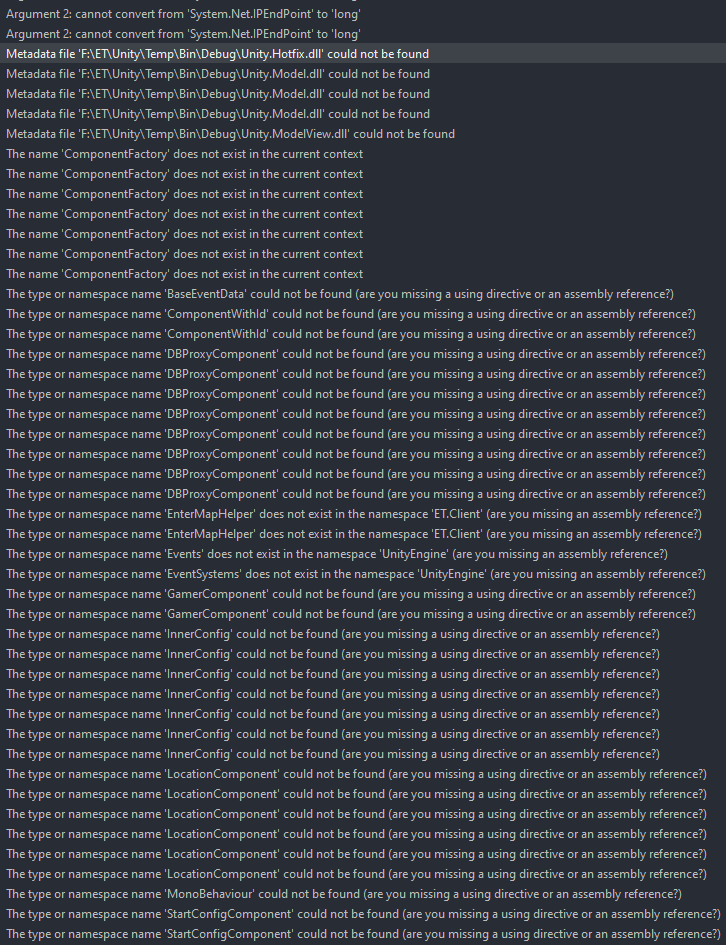
\includegraphics[width=.9\linewidth]{./pic/et4_20230623_152737.png}

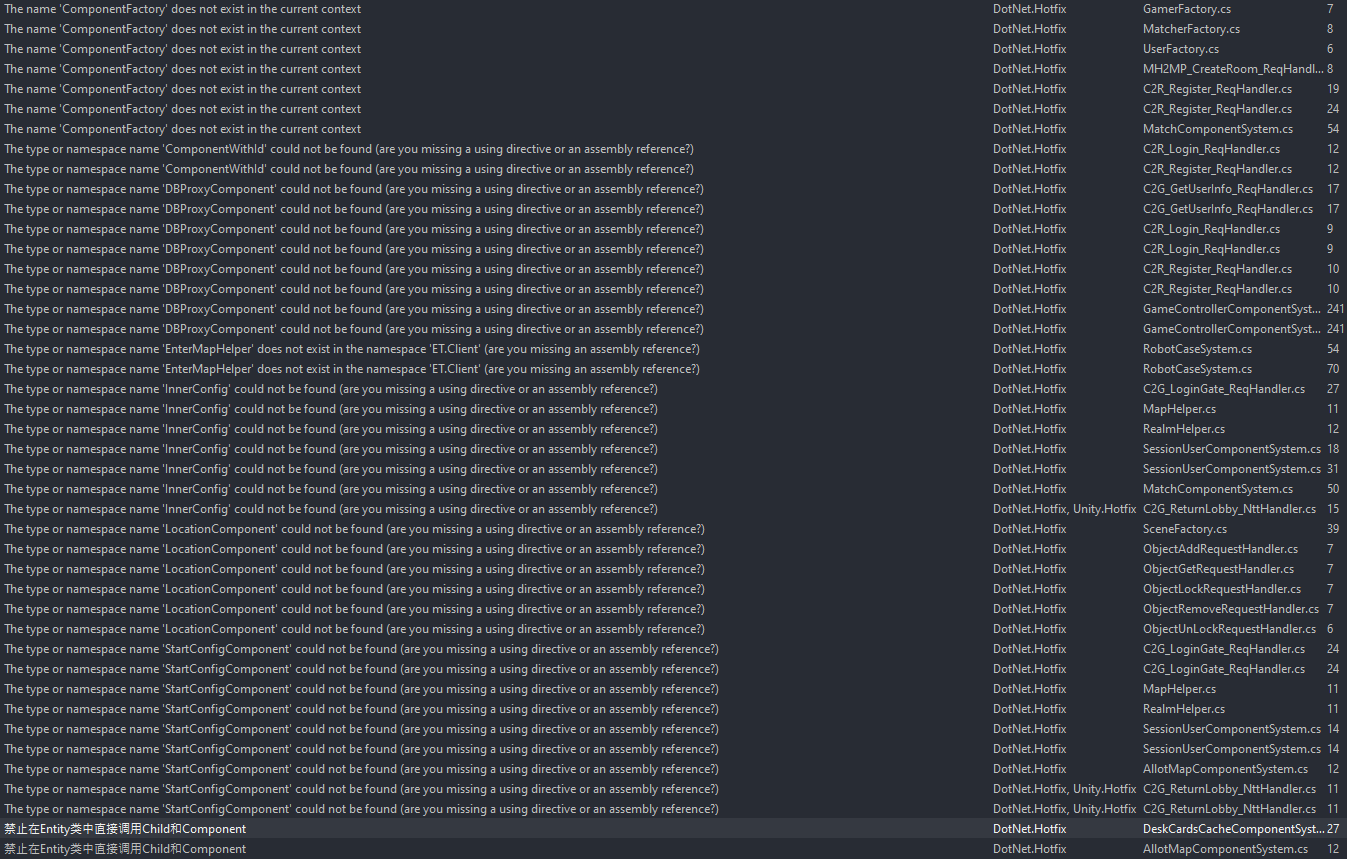
\includegraphics[width=.9\linewidth]{./pic/et4_20230616_165750.png}
\begin{itemize}
\item 【ComponentFactory:】重构了的框架里,这个工厂类是被折解到各自小部件的生产工厂里去了,就是一个框架底层封装的工厂类,拆解到 100 个不同的小部件里。所以我必须得要每个使用的小部件里,它的生产工厂里去再调用相应的逻辑。【可以找个例子出来看一下】
\begin{itemize}
\item Entity 类里面有,组件里添加一个新 new 出来的成员的办法。模仿Player 的使用例子。这里的使用方法是:去拿它的管理组件的实例索引,用管理组件来生成各个元件
\end{itemize}
\item 【PlayerSystem】:不是不知道框架里怎么用,找不出来一个使用的例子吗?它可能不需要用,它只需要框架底层的Entity 里相关方法的封装,能够生成一个一个小单元(Player,Gamer,Matcher-etc)之类的就可以了。就是框架底层原理,这一块儿的,还不太懂
\begin{itemize}
\item 这个工厂类,总是不懂,先去把基类Entity.cs 好好再读一下
\item 同样套用的话,GamerComponent 是房间组件的子组件,拿到这个组件后来创建. VSC 里面好像是有多余的类,所以从 VSC 里看源码,比较乱一点儿。【感觉这一块儿的思路,还没能理清楚。】
\item Hotfix Server \textbf{【UnitFactory】} 生成创建一个单位。可以用作例子。unitComponent.AddChildWithId() 调用的是Entity 里最底封装逻辑。
\begin{itemize}
\item 这个UnitFactory 调用组件方法,来添加进自己的管理系,它所添加的组件是有独特身份ID 的,不适用当前例子
\item 需要去找,自动生成特异性ID, 并创建实例的 Entity 里的方法的例子
\end{itemize}
\item 上面的问题是,如果框架热更新域里可以如上 UnitFactory 一样添加工厂类,那么我的其它小单位Gamer, Player 应该也是可以如上Unit 一样提供他们自己的工厂生产类才对。
\item 再试着多找几个如上的工厂生产类的例子看看。
\end{itemize}
\item \textbf{【ComponentFactory.CreateWithId:】} 重构了的框架里,这个工厂类是被折解到各自小部分的生产工厂里去了,就是一个框架底层封装的工厂类,拆解到 100 个不同的小部件里。所以我必须得要每个使用的小部件里,它的生产工厂里去再调用相应的逻辑。【可以找个例子出来看一下】新框架里,上次不是找到过:先去拿管理器组件,再用管理器组件,通过调用基类Entity 里的方法,来创建小部件的实例?可以再找个例子看一下
\item 上午把【数据库模块的接入】、【InnerConfig】【StartConfigComponent】【LocationComponent】等相关模块:读下源码,理解透彻,必要的情况下下午家里接入并测试
\begin{itemize}
\item 把ActorLocation 相关的,今天晚上一个小时左右,再读一下
\end{itemize}
\item \textbf{【GamerComponent】} :它的逻辑设计应该是什么样的?当服务端有 PlayerComponent 对所有玩家进行管理,当前GamerComponent 只管理一个拖拉机房间里的四个玩家,是RoomComponent 的玩家组成对象(?还有房间组成对象,因为房间如玩家一样需要管理,对应不同拖拉机房间号)$\backslash$
\begin{itemize}
\item 参考项目放在热更新域里面,但是现项目是不允许申明组件放在热更新域里的。去参考项目中其它组件是否全在Model 层申明组件,以及成员变量。暂时把它放到Model 双端共用的地方。
\item 台式机好慢好慢,找了好久才找到这个类。现在应该可以往下改了。这个模块,今天就暂时改到这里,看不见什么相关的编译错误了
\item 这里看出 ET 框架的局限:它把一切成员变量之类的在Model 层里固定死了,也就意味着,热更新是无法热更新功能逻辑模块的重构,只能热更新小细节的实现逻辑。
\end{itemize}
\item \textbf{【GamerComponent 管理类组件】} :逻辑没有理清楚。它是服务端组件,还是客户端组件,还是如PlayerComponent 双端组件,并实现不同的逻辑?
\end{itemize}
\subsection{内网消息等网络相关:请求消息的发送方法等。狠多编译错误,要一点儿一点儿把他们都改掉}
\label{sec-8-3}
\begin{itemize}
\item \textbf{【内网消息等网络相关:请求消息的发送方法等】}: \textbf{在构架里是怎么写的,有几种请求消息的发送方式?}
\item \textbf{明天上午把这块看完,等着我改的编译错误包括} :参考的斗地方游戏里,各种服处理返回消息的逻辑。
\begin{itemize}
\item 因为先前手动发送每个返回消息,我需要将这部分一批消息处理器改为,先试着适配 ET7 框架的重构与底层再封装。
\item 等改过了,真正明白理解了自己重构游戏的需求,再来看去看ET7 框架我要怎么改它现存封装,才能适配自己游戏的需求!!例子:MatchComponentSystem 里的JoinRoom 方法等相关逻辑。
\item 【下午还没有改到这里来。先从简单的改起,因为一个热键的优化,感觉VS 好用一点儿了。先能改多少改多少,再按模块来改像消掉所有的ETTask 相关一样把一个模块的所有的编译错误全部改完!!!】
\end{itemize}
\item 去看上面列过的那个例子MatchComponentSystem, 参考项目里的各种服的消息处理,怎么适配成ET7 重构后的不用手动发返回消息(发送过程封装在框架底层),和记录可能存在的问题(某些服的逻辑,返回消息的发送时间与其它必要逻辑,顺序变得重要的时候,记下来,晚点儿会再重构ET7 框架适配游戏需求)
\end{itemize}
\subsubsection{修改下面的ActorMessageSenderComponent 因为功能模块逻辑重构,而带来的一堆编译错误。}
\label{sec-8-3-1}
\begin{itemize}
\item 修改方法过程步骤:去框架里搜索,其它任何地方发送消息的例子,看 \textbf{【重构后的框架是如何发送消息的, Call() Send() 方法的调用等】} 这个明天上午一定看,因为不懂,不会改怎么发送消息的()
\item 然后参照例子,把客户端和必要的小服里,所有需要发送消息的地方,改成上面看到总结的发送方法里。
\end{itemize}

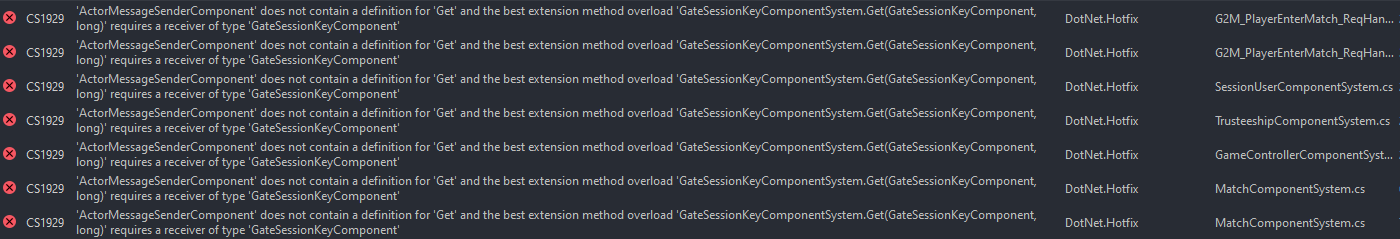
\includegraphics[width=.9\linewidth]{./pic/et4_20230616_160327.png}

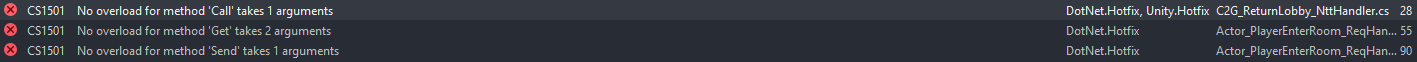
\includegraphics[width=.9\linewidth]{./pic/et4_20230616_165027.png}
\begin{itemize}
\item 【地图服Unit 相关】:先前所有接触到这个框架,都只看了个头,就是只限于能够任何客户端连接到服务端能够注册登录的程度,后面的其它服、框架逻辑全都还不曾看。所以今天上午扫一眼地图服相关,是糊的。要把这些前前后后相关的原理总弄懂了。
\item 去框架里搜发送的调用方法,可能现在 Mac 系统里有一点儿障碍的,就是VSC 不报错,不知道搜出来的是对的,还是错的。但是几种不同的方法,先总结在这里,对照运行时的报错一一改过来。必须把这块儿弄明白了。【爱表哥,爱生活!!!任何时候,活宝妹就是一定要嫁给亲爱的表哥!!爱表哥,爱生活!!!】
\item 【拿到Session 会话框,调用其Send() 方法】:例子 PingComponentAwakeSystem 里的 PingAsync() 方法。它是一个心跳包。这个心跳包就是一Awake() 醒来,全生职责就是周期性给服务器发消息
\item 然后参照例子,把客户端和必要的小服里,所有需要发送消息的地方,改成上面看到总结的发送方法里。
\item 框架里,各种不同场景下发送消息的方法:
\item 【场景里拿到SessionComponent】,调用会话框的发送方法Send()
\begin{minted}[fontsize=\scriptsize,linenos=false]{csharp}
robotScene.GetComponent<Client.SessionComponent>().Session.Send(new C2M_TestRobotCase2() {N = robotScene.Zone});

// 也可以借助UnitGateComponent 拿到它的成员变量 GateSessionActorId, 用这个可以重构后发消息
ActorMessageSenderComponent.Instance.Send(u.Unit.GetComponent<UnitGateComponent>().GateSessionActorId, message);
\end{minted}
\item 【活宝妹任何时候就是一定要嫁给亲爱的表哥!!!】迷迷糊糊地把一个模块改完了,可是感觉那个改掉的模块,像是还没能理解透彻。明天上午会再看一下。【爱表哥,爱生活!!!任何时候,亲爱的表哥的活宝妹,就是一定要嫁给亲爱的表哥!!爱表哥,爱生活!!!】70 Compile Errors 还没有改完,涉及功能模块人接入与整合。会明天上午看过读一下相关模块的源码后再试着改。【活宝妹就是一定要嫁给亲爱的表哥!!!爱表哥,爱生活!!!】
\end{itemize}
\subsubsection{【ActorMessageSenderComponent】:这个类狠重要、狠重要,现在是活宝妹理解网络模块的核心。爱表哥,爱生活!!!}
\label{sec-8-3-2}
\begin{itemize}
\item 得去想:ActorMessageSenderComponent, 是只能用来处理跨进程消息的吗?普通消息的发送是如何处理的?该弄明白,它的适用范围,适用哪些情境上下文
\item \textbf{【ActorMessageSenderComponent】} :因为ET7 这个模块的重构。不再需要每个返回消息手动去拿消息发送器,交由框架底部去处理。
\item 不懂的是,如何重构,消除参考项目里各种服的消息处理里,怎么适配成ET7, 不用去拿消息发送器,只把返回消息结果写好,或是发送(请求)消息时,如何发送?
\item 不同于昨天上午看过的,NetInnerComponentOnReadEvent 是对上层读到消息后的处理,就是消息已经准备好了,甚至已经通过某种逻辑代理,到达和触发了NetInnerComponentOnRead 事件了(这个事件是怎么触发的?大概是,每个进程会有一个内网组件NetInnerComponent. 当内网组件读到消息会触发。读到消息,包括本进程消息,也就包括,由其它进程发回来的返回消息。这个,可能更底层Session 发回来跨进程消息的地方?改天去捡)。现在要去理解的是,比如发送一条请求消息,创建一个请求消息实例后,如果运动可以走到上面的触发读到消息事件?就是消息流程的前半部分。NetInnerComponentSystem.cs 的读到消息事件,要再往前看一点儿。
\item 把消息的处理流程几个重要的方法 \textbf{【ActorMessageSenderComponentSystem Send() Call() 等】} ,这里再梳理一遍:
\end{itemize}
\begin{enumerate}
\item ActorMessageSenderComponentSystem Send():
\label{sec-8-3-2-1}
\begin{itemize}
\item 【任何时候,活宝妹就是一定要嫁给亲爱的表哥!!!活宝妹若是还没能嫁给亲爱的表哥,活宝妹就永远守候在亲爱的表哥的身边!!爱表哥,爱生活!!!】
\item 今天终于把里面的计时器原理看懂了。
\item \textbf{【ActorMessageSenderComponentSystem Send()】} 发的是普通消息(不是不需要回复消息,是任何消息,都走这一步,因为是最基的基类接口)
\begin{itemize}
\item 【同一进程消息】:不走网络层,直接交由本【进程?】的消息处理器处理。就是(ActorMessageSenderComponentSystem Send()里)判断如果是同一进程,它会调用内网组件处理消息:NetInnerComponent.Instance.HandleMessage(actorId, message); 【注意这里是一个进程内网组件消息的一个来源:本进程消息。它同样接收和读来自其它进程的消息,跨进程消息】。而内网组件的这个HandleMessage() 静态方法,就发发布内网组件读到消息事件;内网组件读到消息事件的发布,会触发调用 NetInnerComponentOnReadEvent 借助 ActorHandleHelper 来处理内网消息。后面的就是昨天上午读到的部分。这里的疑问就是:谁,哪里调用发送组件的Send() 发送事件?
\item 【不是同一进程消息】:就通过内网组件,去拿同那个收消息进程的会话框,通过会话框走Session 流程发跨进程消息。就是走网络层。
\end{itemize}
\end{itemize}
\item ActorMessageSenderComponentSystem Call()
\label{sec-8-3-2-2}
\begin{itemize}
\item \textbf{【ActorMessageSenderComponentSystem Call()】} 发的是要求返回结果的消息:返回 ETTask<IActorResponse>
\begin{itemize}
\item 注意 \textbf{【跨进程消息的回复细节里】} ,看见IRpcResponse 实例创建好,结果写好,同步到异步任务ETTask 里,总容易忘记ETTask 的异步任务运行结束(如果不是抛异常), \textbf{跨进程消息是如何回到消息的发送进程的?} 是AMRpcHandler 抽象类里,异步等待实体实现类里的具体实现逻辑Run() 异步方法执行结束,也就是等待各种消息处理服处理好、写好异步返回消息IRpcResponse, 同步到异步任务ETTask. AMRpcHandler 抽象类里等异步方法执行完成,抽象类里作了封装,把返回消息通过进程间通信会话框,把返回消息发回去的。
\item 这里看见,这个消息发送器底层逻辑说,如果是我自己进程要发消息,就封装消息发送者 rpcId 是自已的 rpcId. 然后调用自组件Call() 发送消息。后面的几个方法,大概就是跨进程消息的发送与回复。
\end{itemize}
\end{itemize}
\end{enumerate}
\subsection{静态类的环形引用问题}
\label{sec-8-4}
\begin{itemize}
\item 静态类 CardsHelper, 与静态类 DeskCardsCacheComponent.System 之间,存在静态类的互相引用:就是说,两个静态类,互相引用了对方的方法
\begin{itemize}
\item CardsHelper 里,引用了DeskCardsCacheComponent.System 里的方法
\item 而 DeskCardsCacheComponentSystem 类里,同样引用了 CardsHelper 里的方法
\item 我的解决办法是:热更域里的 DeskCardsCacheComponentSystem 对CardsHelper 类里引用的两个静态方法,直接复制了一份在 DeskCardsCacheComponentSystem 类里面,就可以消除了。再次体验VS 的显著延迟,真让人受不了。是因为这个软件被监控吗?
\end{itemize}
\end{itemize}
\subsection{下面是已经改好了的:还是先放着,备查}
\label{sec-8-5}

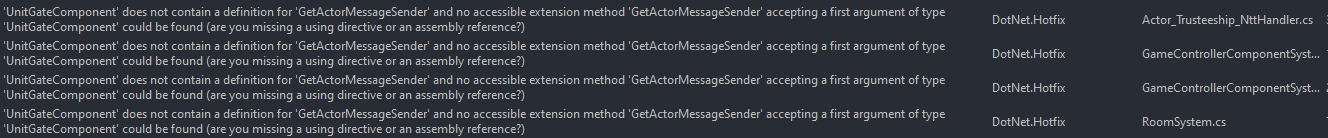
\includegraphics[width=.9\linewidth]{./pic/et4_20230616_162711.png}
\begin{itemize}
\item 【UnitGateComponent]: 怎么才能成为多个不同组件的组成部分?
\end{itemize}

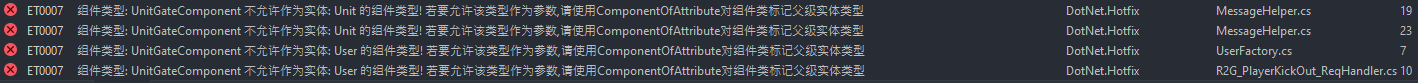
\includegraphics[width=.9\linewidth]{./pic/et4_20230616_165317.png}
\begin{itemize}
\item 【解决办法】:去查框架里的源代码,写得极其清楚:
\begin{minted}[fontsize=\scriptsize,linenos=false]{csharp}
// 组件类父级实体类型约束
// 父级实体类型唯一的 标记指定父级实体类型【ComponentOf(typeof(parentType)】
// 不唯一则标记【ComponentOf]
[AttributeUsage(AttributeTargets.Class)]
public class ComponentOfAttribute : Attribute {
    public Type Type;
    public ComponentOfAttribute(Type type = null) {
        this.Type = type;
    }
}
\end{minted}
\begin{itemize}
\item 所以上面的解决办法就是:不要标记 typeof 参数就可以了呀,它就可以成为多个不同组件的子元件部件了呀。。。是这样的
\end{itemize}
\begin{minted}[fontsize=\scriptsize,linenos=false]{csharp}
[ComponentOf] 
public class UnitGateComponent : Entity, IAwake<long>, ITransfer, ISerializeToEntity { // 不知道这里为什么会受到限制,这里再改一下
    public long GateSessionActorId { get; set; }
    // 想一下,下面的变更还需要吗?要不要,是看框架里有没有什么,自动上线自动下线处理之类的,相关的?
    public bool IsDisconnect;
}
\end{minted}
\end{itemize}
\subsection{先前列的相对杂一点儿}
\label{sec-8-6}
\begin{itemize}
\item 【问题】:上次那个ET-EUI 框架的时候,曾经出现过 opcode 不对应,也就是说,我现在生成的进程间消息,有可能还是会存在服务器码与客户端码不对应,这个完备的框架,这次应该不至于吧?
\item 【UIType】部分类:这个类出现在了三四个不同的程序域,现在重构了,好像添加得不对。要再修改
\item \textbf{【ET7 框架】} 没有处理的逻辑是: \textbf{【ET7 框架里数据库的接入】}
\item \textbf{【UILobbyComponent 可以测试】} :这个大厅组件,Unity 里预设简单,可以试运行一下,看是否完全消除这个UI 组件的报错,这个屏的控件能否显示出来?还是错出得早,这个屏就出不来已经报错了?
\begin{itemize}
\item 【客户端】的逻辑是处理好了,编译全过后可以测试
\item 【服务端】:处理用户请求匹配房间的逻辑,仍在处理: \textbf{C2G\_StartMatch\_ReqHandler}.
\end{itemize}
\item \textbf{【TractorRoomComponent】} :因为是多组件嵌套,可以合并多组件为同一个组件;另早上看得一知半解的一个【ChildOf】标签,可以帮助组件套用吗?再找找理解消化一下
\item 【房间组件】:几个现存的 working-on 的问题:
\begin{itemize}
\item 多组件嵌套:手工合并为一个组件。彻底理解确认后,会合并
\item 【服务端】:处理用户请求匹配房间的逻辑. 这里的编译错误终于改完。到时就看运行时错误了。
\begin{itemize}
\item 【数据库模块的整合】:网关服在转发请求匹配时,验证会话框有效后,验证用户身份时,需要去【用户数据库】拿用户数据。ET7 留了个DBManagerComponent, 还没能整合出这个模块
\end{itemize}
-【参考来源 \textbf{C2R\_LoginHandler} 】:Realm 处理客户端的登录请求的服务端逻辑。这里看见,它随机分配一个网关服。也就是,我(原本本质上也是随机分配)一个匹配服给用。可以依照这里的例子来改写。
\end{itemize}
\item 【匹配服地址】网关服的处理逻辑里,验证完用户合格后,为代为转发消息到匹配服,但需要拿匹配服的地址。ET7 重构里,还没能改出这部分。服务器系统配置初始化时,可以链表管理各小构匹配服,再去拿相关匹配服的地址。ET7 框架里的路由器系统,自己还没有弄懂。
\item \textbf{【ET7 IMHandler 对回复消息的写封装, 与自动回复消息的封装】} :可能无法处理游戏过程中的某些逻辑。就是涉及到一定顺序,尤其需要先回复消息的处理服处理逻辑。举例:C2G\_StartMatch\_ReqHandler. 所以,这里要自己好好想透彻一点儿。要如何改,才能适配自己游戏的需求。
\item \textbf{【 ComponentFactory:】} ET7 里重构,被分布到各种不同的组件里去了。想复制个文件过来,把与之相关的全部消掉,但因为大规模重构,复制了文件也没用。总之ET7 就是感觉什么乱七八糟的,感觉他们大规模糊乱重构的目的就是故意挫败人。可是这个世界上就偏偏存在亲爱的表哥的活宝妹这样的不服的!!!爱表哥,爱生活!!!任何时候,活宝妹就是一定要嫁给亲爱的表哥!!!爱表哥,爱生活!!!

\item \textbf{【PlayerComponent 类重复】} : 狠奇怪:删除了说找不到类,不删除说重复了,感觉台式机应用有延迟?反应狠慢。。。。。文件嵌套想要显示所有嵌套文件的时候,要狠久狠久重启好几次才反应得过来
\begin{itemize}
\item 原本有两个类都是如上面这个类这样,但有时候台式机反应稍快一点儿,就是一个类找不到出现上面的情况。破电脑的延迟反应,弄得我都要怀疑VS 应用被别人操控了。。。
\item 【爱表哥,爱生活!!!任何时候,活宝妹就是一定要嫁给亲爱的表哥!!!爱表哥,爱生活!!!】
\end{itemize}
\item 把还没有用到,但是报错了的几个类删掉:比如记一下: SessionInfoComponent,
\begin{itemize}
\item 还剩最后 26 个最挑战活宝妹的编译错误,今天傍晚会家里改会儿,集中问题明天上午希望能够看懂。【爱表哥,爱生活!!!任何时候,活宝妹就是一定要嫁给亲爱的表哥!!】
\end{itemize}
\end{itemize}

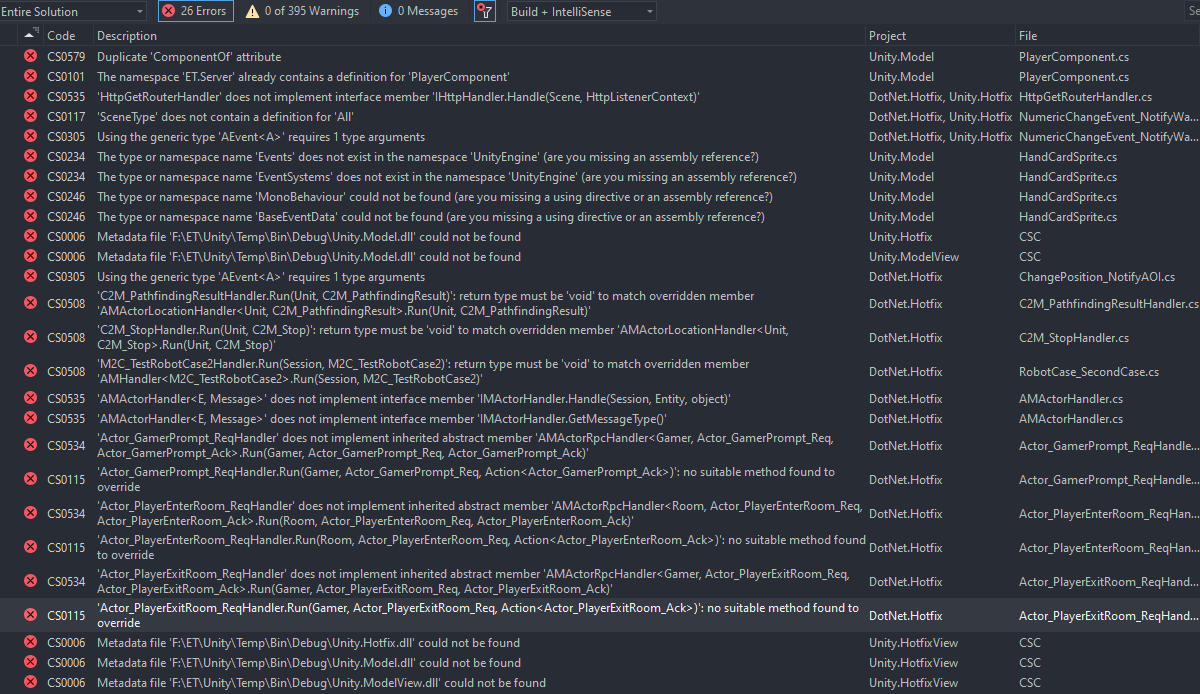
\includegraphics[width=.9\linewidth]{./pic/et4_20230604_162732.png}
\begin{itemize}
\item 把Root 根场景以及启动时添加的组件大致看了一遍。想把上面的消息处理器再系统化地看一遍,理解一下,总改不到这个模块相关的编译错误。
\item \textbf{【ETTask ETVoid 是必须弄懂的】} ;看两个小时,像昨天晚上一样真正投入进去看。我相信自己看得懂,弄得透,只是需要投入一点儿时间。
\begin{itemize}
\item 感觉前一个周左右的时间,倍受睡眠困扰。活宝妹做梦也不会想到,昨天的自己会困成那个样子(感觉开1 小时的车极度困难,太容易睡着。。)。。现在试着一再调整状态,少喝咖啡多运动,最重要的,仍是把学习的状态调整出来调整回来。至少学到活宝妹可以嫁给亲爱的表哥的这一天!!!
\item 这个异步的原理,感觉是弄明白了,今天上午又看了一遍看了会儿。下午去改那些 IMHandler, 希望今天下午能够改彻底。就是真正弄明白了去改(现在的问题就是,几个IMHandler 的实体实现类,改天这个顾不了那个,没弄明白,接口方法怎么申明定义,才能兼顾所有实例类消息处理器?),不是只改掉了当前的编译错误,等真正运行的时候,一个个运行错误或是异常往外冒!!!今天脑袋还算清醒,下午好好弄弄这个
\end{itemize}
\item 【爱表哥,爱生活!!!任何时候,亲爱的表哥的活宝妹,都是一定要嫁给亲爱的表哥的!!!】【三楼上的贱鸡贱畜牲真多!!!一天到底没想点儿好的】活宝妹还没能嫁给亲爱的表哥,活宝妹就是永远守候在亲爱的表哥的身边!!!爱表哥,爱生活!!!
\item 再然后 ,再看下下面的 UnitGateComponent 相关。下午或傍晚有时间的时候,可以再折腾折腾 emacs-org-mode 下划线删除字体设置为斜体。
\item \textbf{【UnitGateComponent】} 加个方法用?可能不需要加方法;另一个错是,不能同时成为两个不同 entity 的子控件?【ComponentOf(typeof(Unit))】etc 出错文件在 (C2G\_EnterMapHandler)
\begin{itemize}
\item 这里要把 ActorMessageSenderComponent 组件给弄明白。它有个有序管理字典,记着 actorId 与ActorMessageSender 的一一对应关系,就可以封装维护消息的自动发送等,以及必要的超时消息管理。
\end{itemize}
\item \textbf{【服务端Actor\_PlayerEnterRoom\_ReqHandler 这个处理类】} 现在还很多问题,需要弄懂,往下改
\item 今天晚上会把刚才下午看见、意识到几个模块的问题试着分析明白,记下笔记。
\item \textbf{ETTask-vs-ETVoid}: 框架里有狠多需要改的地方。今天上午的脑袋好使,把这块儿再仔细好好看下。今天上午把以前不懂的模块都稍微看下,再理解一下
\begin{itemize}
\item 查网页感觉也查不出什么来。还是用源码帮助理解概念。【爱表哥,爱生活!!!活宝妹就是一定要嫁给亲爱的表哥!!!】
\item 不能把所有基类的 async ETTask 返回参数直接改成 void, 因为框架的顶层应用,服务端或是客户端,当不异步等待结果,如资源包没能下载完成,就接着往下执行,会报空异常。
\end{itemize}
\item 现在的问题是:Protobuf 里 repeated 关键字,好像还是没有处理好,找不到成员变量  Cards. 是因为 Proto2CS 的时候,确实把 repeated 关键字给处理丢了。因为我的 .proto 文件里有错误。(这就是上面先前觉得奇怪的原因。因为改这个的过程中把那些错改正了,就可以生成成功并找到相关的消息了)。
\item 这部分总感觉弄得不是狠透彻。就再花点儿时间。这段时间产量太低,可以先试着完成其它模块。
\item \textbf{【HandCardSprite 这个最近要弄明白】} 不知道这个类是为什么,整了一堆的错误,它是ETModel 里的。感觉是常规域,没弄明白为什么常规域还有ILRuntime 的适配呢?
\begin{itemize}
\item 要把 ILRuntime 热更新第三库,也再弄得明白一点儿【今天上午把这里再看,最好是能够结合源码看看】为什么这个类还要适配ILRuntime ?
\item 这里这个类,整个框架里只找到这一个用的地方,所以它一定是添加在某个预设或是场景中的某个控件下的。只是参考项目的unity 客户端,我运行不到打牌的这个界面,就先因为抛出异常而淡能运行。所以还没能找到哪个预设或是场景中的哪个控件添加了这个类,但是当然一定是跟玩家手牌相关的。 \textbf{【HandCardSprite 是在 handcard 预设里添加了这个脚本】}
\item 这个类今天运行狠奇怪,VS022 里找不到了。。。就是说,VSC 里它是在Model 客户端的源码里,但是从VS 里打开,找不到这个类文件所在的文件夹和文件,没有索引好,再添加一下?
\item 那么,为什么前两天被这个 block 住,而那天,好像是有删除掉这个文件,但文件夹应该是还在的才对呀?我可能还会试着再把它添加回去。
\item 但是,会在把当前几个编译错误改完,试着测试一下客户端现在有的界面之后,再试着添加回去,整理和 develop TractorRoomComponent 界面的内容。【爱表哥,爱生活!!!活宝妹任何时候就是一定要嫁给亲爱的表哥!!】
\item 今天下午家里再运行一次,当客户端抛异常,应该是某个热更新的资源包没有找到什么的?所以可以试着自己去解决这个客户端实时运行时抛出的异常。
\item \textbf{【参考项目斗地主客户端异常】} :再运行一次,试着分析,是否可以 unity 里实时运行,如果不可以,为什么不可以?
\begin{itemize}
\item 应该是LandlordsRom 这个预设与UI 类型没能连接起来,也就是找不到这个预设。
\item 那为什么打好包的可以呢?因为打好包的预设包名 LandlordsRoom.unity3d 与游戏逻辑契合,可以找得到
\item 可是仍然感觉奇怪:LandlordsLogin 与LandlordsLobby, 非常类似都可以找到,为什么就LandlordsRoom 找不到?可能LandlordsRoom 预设还是有某点儿物对特殊的地方。
\item 上面这个暂时跳过。现在仍然主要去看HandCardSprite 为什么参考项目里可以,而ET7 里就不可以。
\end{itemize}
\item 就是上面那个异常,今天下午得去弄明白,为什么只在 unity 实时运行时会抛异常,而如果是三个打包好的客户端,就不会。也就是说,打包好的不存在找不到类、找不到预设、或是找不到任何相关资源的问题。
\item 这个项目Unity.Model 是需要索引 UnityEngine 以及UI 等相关模块人的 .dll 的。暂时还没弄明白它是怎么加的
\item 【爱表哥,爱生活!!!任何时候,活宝妹就是一定要嫁给亲爱的表哥!!】
\end{itemize}
\item \textbf{ClientComponent} 参考项目组件:去看ET7 里客户端的 PlayerComponent.
\item 【爱表哥,爱生活!!!任何时候,活宝妹就是一定要嫁给亲爱的表哥!!!】今天下午先去看 Tractor 游戏源码,设计重构思路
\item 【活宝妹坐等亲爱的表哥,领娶活宝妹回家!爱表哥,爱生活!!!】
\item \textbf{【亲爱的表哥,这个世界上,只有一个活宝妹,这么心心恋恋,就是一定要嫁给亲爱的表哥!!!问世间情为何物,直教人生死相许。。亲爱的表哥,一个温暖的怀抱拥抱的魂力可真大呀,管了这如许多年!!这不,你的活宝妹为了这个温暖的怀抱拥抱,就是一定要嫁给亲爱的表哥!!不嫁就永远守候在亲爱的表哥的身边!!爱表哥,爱生活!!!活宝妹就是一定要嫁给亲爱的表哥!!!】}
\item 亲爱的表哥,活宝妹相信舅舅十岁闯江湖的阅历,活宝妹深深相信亲爱的表哥。活宝妹就是稳稳地永远守候在亲爱的表哥的身边!爱表哥,爱生活!!!活宝妹就是一定要嫁给亲爱的表哥!!
\item 【爱表哥,爱生活!!!任何时候,活宝妹就是一定要嫁给亲爱的表哥!!!】
\end{itemize}
\subsection{LocationComponent: 【任何时候,亲爱的表哥的活宝妹就是一定要嫁给亲爱的表哥!!!爱表哥,爱生活!!!】}
\label{sec-8-7}
\begin{itemize}
\item 【今天上午】:从这里开始,把先前总结 Actor 消息以及处理器时,所有关于位置的消息,以及相关的消息处理器弄懂。【没看完】
\begin{itemize}
\item 先前,消息处理器的部分,只看了一个接口类和两个抽象实现,其它没看
\item 消息,位置消息相关的内容,还没看不懂。
\end{itemize}
\item 【亲爱的表哥,活宝妹一定要嫁的亲爱的表哥!!任何时候,活宝妹就是一定要嫁给亲爱的表哥!!爱表哥,爱生活!!!】
\item 【任何时候,亲爱的表哥的活宝妹,就是一定要嫁给亲爱的表哥!!!爱表哥,爱生活!!!】任何时候,活宝妹还没能嫁给亲爱的表哥,他们就大可不必发疯犯贱。任何时候,他们发疯犯贱,他们也永远只能是发疯犯贱得了一时,发疯犯贱不了一世。亲爱的表哥的活宝妹,若是还没能嫁给亲爱的表哥,亲爱的表哥的活宝妹,就是永远守候在亲爱的表哥的身边!!爱表哥,爱生活!!!
\item 因为框架狠大,是一个大型网络游戏双端框架,因为内容比较多,现在已经总结的是四个文件,还要常作笔记,否则容易忘记,前后不连贯。所以难免小细节的地方,没能注意到,没什么大不了
\item 这个模块的编译错误,被活宝妹全部给消除掉了。。。
\end{itemize}
\subsection{【HandCardSprite.cs】}
\label{sec-8-8}
\begin{itemize}
\item \textbf{【HandCardSprite.cs】} :这个客户端文件里存在一堆关于Unity 引用的错误。把这个有着巨多错误的类重新添加到了框架里。现在着眼着这些错误(加了这个文件,错误又多了二三十个!!!)。
\begin{itemize}
\item \textbf{【参考项目Game.cs】} 客户端类里,存在UnityEngineer 的诸多引用,所以HandCardSprite.cs 可以通过Game.EventSystem 等拿到引用。但ET7 重构得没有边际。必须自己去看明白。这个类,更多的是,适配特定游戏需求的ET7 框架外的一个桥梁适配类。
\item 【参考项目热更域里的 Game.cs 类】:
\begin{minted}[fontsize=\scriptsize,linenos=false]{csharp}
public static class Game {
    private static Scene scene;
    public static Scene Scene {
        get {
            if (scene != null) 
                return scene;
            scene = new Scene();
            return scene;
        }
    }
    private static EventSystem eventSystem; // <<<<<<<<<<<<<<<<<<<< 
    public static EventSystem EventSystem {
        get {
            return eventSystem ?? (eventSystem = new EventSystem());
        }
    }
    private static ObjectPool objectPool; // <<<<<<<<<<<<<<<<<<<< 
    public static ObjectPool ObjectPool {
        get {
            return objectPool ?? (objectPool = new ObjectPool());
        }
    }
    public static void Close() {
        scene.Dispose();
        scene = null;
        eventSystem = null;
        objectPool = null;
    }
}
\end{minted}
\end{itemize}
\item 现框架里不存在的,需要整合进来的模块版块:DBProxyComponent, InnerConfig, LocationComponent, StartConfigComponent
\item 组件管理类:某些组件,属于双端,但客户端与服务端的逻辑不一样,如PlayerComponent; 某些组件,只属于服务端;有只属于客户端的吗?
\end{itemize}
\subsection{【数据库模块:】}
\label{sec-8-9}
\begin{itemize}
\item 把IMHandler 接口,以及它的两个抽象实现类、相关模块的部分理解透彻
\item 先看只看了一半的,比如什么IMHandler 接口的实现类等,如果今天上午有机会,也可以看一下
\item InnerConfig 和 StartConfigComponent 也都稍微看一下:感觉 ET7 重构后,这些自己基础相对欠缺的模块,还没仔细看
\item 【任何时候,活宝妹就是一定要嫁给亲爱的表哥!!!】现在编译错误还剩几个模块
\end{itemize}
\subsection{IPEndPoint-to-long 转化}
\label{sec-8-10}
\subsection{两件杂事:}
\label{sec-8-11}
\begin{itemize}
\item 【先花 10 分钟左右,搜下看 emacs-export-to-pdf 与 Skim 应用的自动同步,能理解回调适配过程吗?】还是比较麻烦,改天傍晚或是晚上再凭兴趣来解决,早上看别的
\begin{itemize}
\item 这里主要的问题时,Skim 实时更新外源 pdf 的更新时,因为 emacs 的 export-to-pdf 有个过程,这个过程中生成 table-of-contents 比较靠后,如果不背便条,就必须得每次重点查看TOC. \textbf{Skim 怎么才能够接收到 latex 生成TOC 完成后的回调,来从 Skim 中显示 TOC?}
\item 这里要去想,为什么背个便条,就能最终自动显示 TOC 了呢?背便条能够最终显示 TOC 是为什么, \textbf{背便条背后的原理,能否借用} ?
\item 另外,【可以考虑, \textbf{过滤掉或是配置掉背便条自动同步过程中的确认窗口繁琐过程} 】如果每个 pdf 的自动生成与刷新,我不需要多次点 enter 确认窗口,我只需要点击一个,或者甚至一个也不需要点,就也算满足用户需求。
\end{itemize}
\item VSC 的配置可能哪里写得不对。以前没有这个问题。现VSC 跳转至 emacs 打开当前 buffer, 不能精确定位到 VSC 中当前 buffer 所在的行。改天有机会的时候再 debug 一下。
\end{itemize}
\subsection{StartConfigComponent: 现框架里有重构了的版本,在理解现ET7 框架的基础上进行必要适配:先把之前总结的再熟悉一下,下午有时间也看看这个}
\label{sec-8-12}
\begin{itemize}
\item InnerConfig: 可以把老版本里的 InnerConfig 类,参考对比ET7 里的ConfigSingleton<T> 泛型类,来试着理解和适配这相模块。因为同属配置类,就是分两个模块。
\item 昨天看了大半天StartConfigComponent 等配置相关,现在感觉看不出什么来。下午带适配任务,把这两三个相关的模块改完。晚上回学校学习。
\end{itemize}
% Emacs 28.2 (Org mode 8.2.7c)
\end{document}